\section{Systematic uncertainties}
\label{sec:syst}

In this chapter we present and evaluate the systematic uncertainties associated 
to the polarization measurements reported in the previous chapter.

After considering several potential sources of systematic uncertainties,
we converged on the following list, which will be discussed in detail in the next sections.
\begin{itemize}
\item Potential differences between the 2017 and 2018 samples;
\item Fit model of the dimuon mass distributions;
\item Single muon detection efficiencies;
\item Dimuon detection efficiencies (``$\rho$ factor");
\item Potential residual azimuthal anisotropy in the helicity frame.
\end{itemize}

\subsection{Potential differences between the 2017 and 2018 samples}

To study the impact of possible differences between the 2017 and 2018 event samples,
we measured the prompt \jpsi polarization independently in each sample.
As can be seen in Fig.~\ref{fig:2017vs2018}, for the \jpsi and \psip cases,
the two measurements are compatible with each other, 
within their (independent) statistical uncertainties.
We could consider this to be a ``passed check" but, to be conservative, 
we will assign a systematic uncertainty of $\pm 0.012$, independent of \pt,
to this effect. This uncertainty is represented in the figures by the pink band.

\begin{figure}[h]
\centering
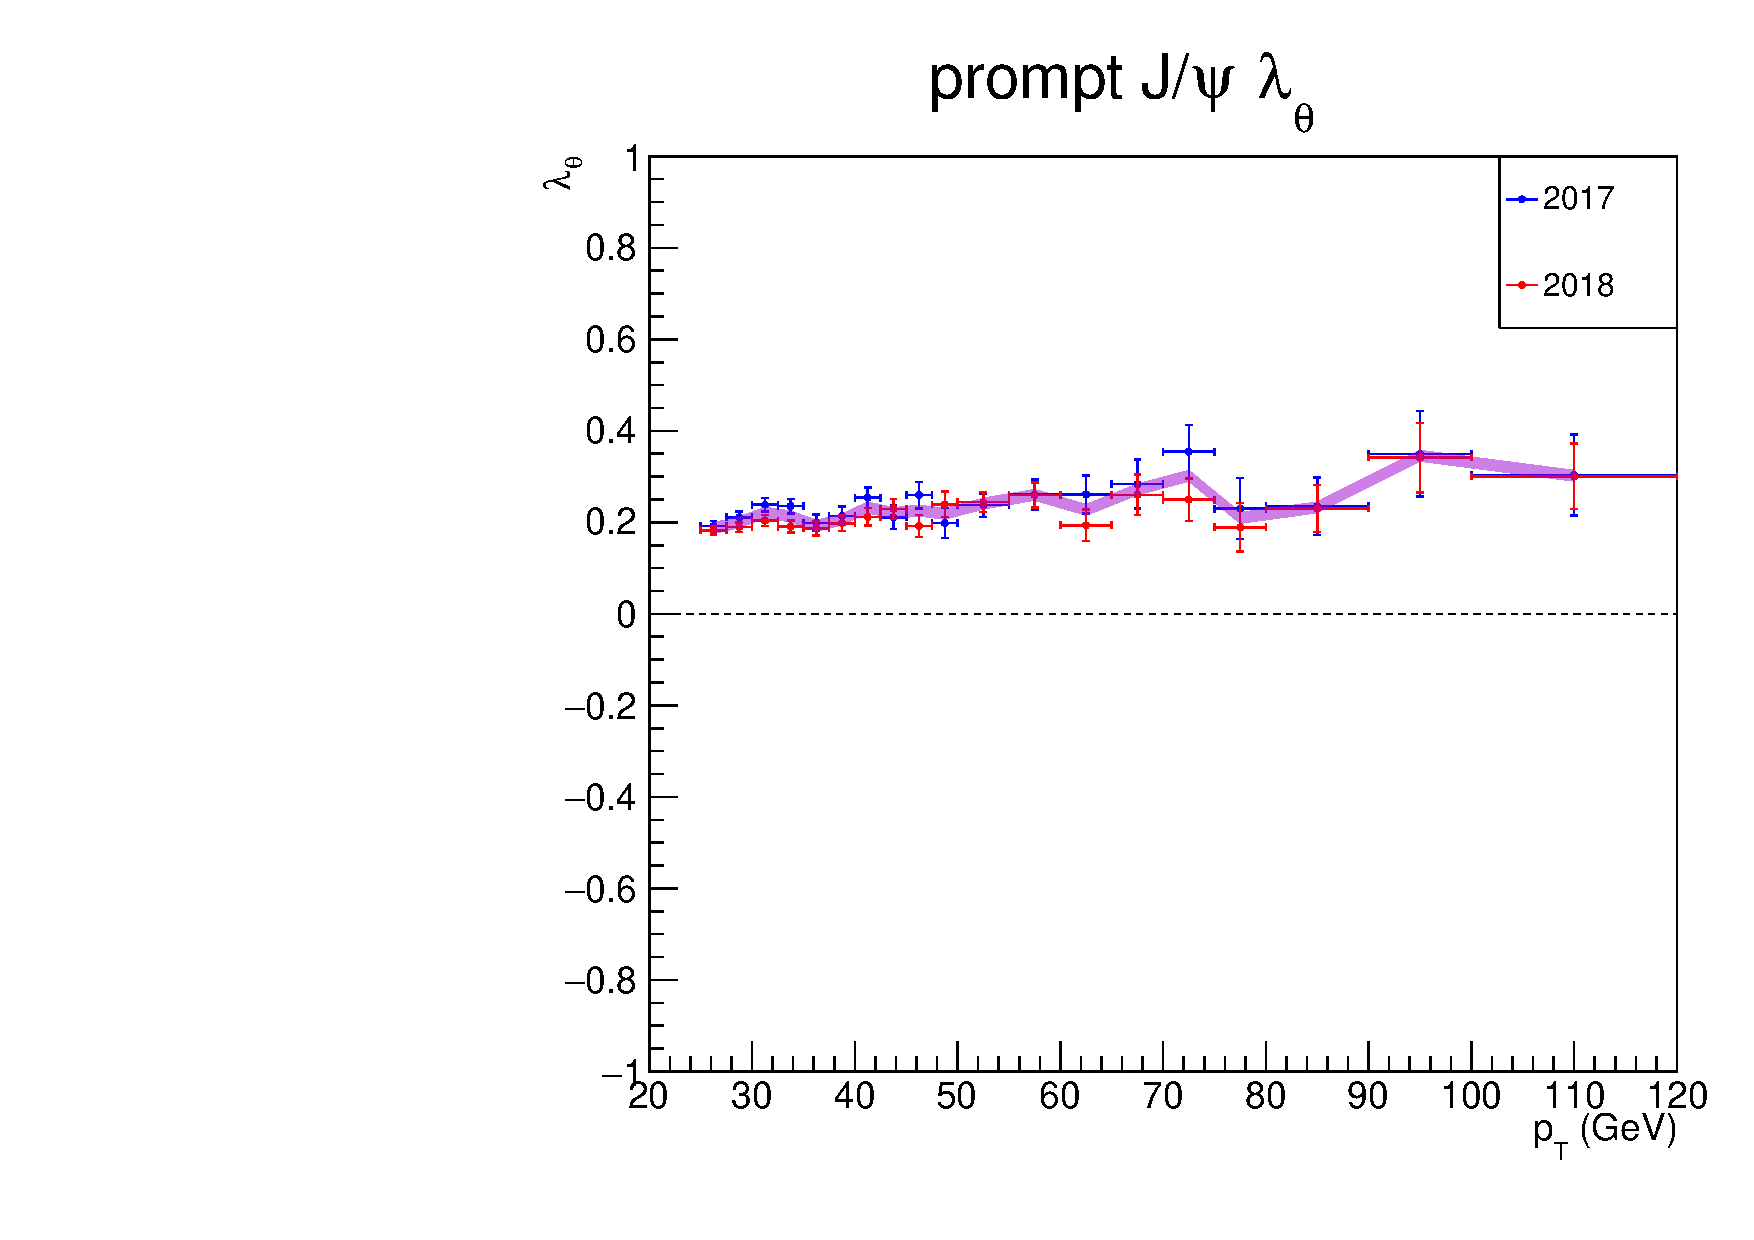
\includegraphics[width = 0.48\textwidth]{Figures/chapter6/par_lth_years_unc-jpsi.pdf}
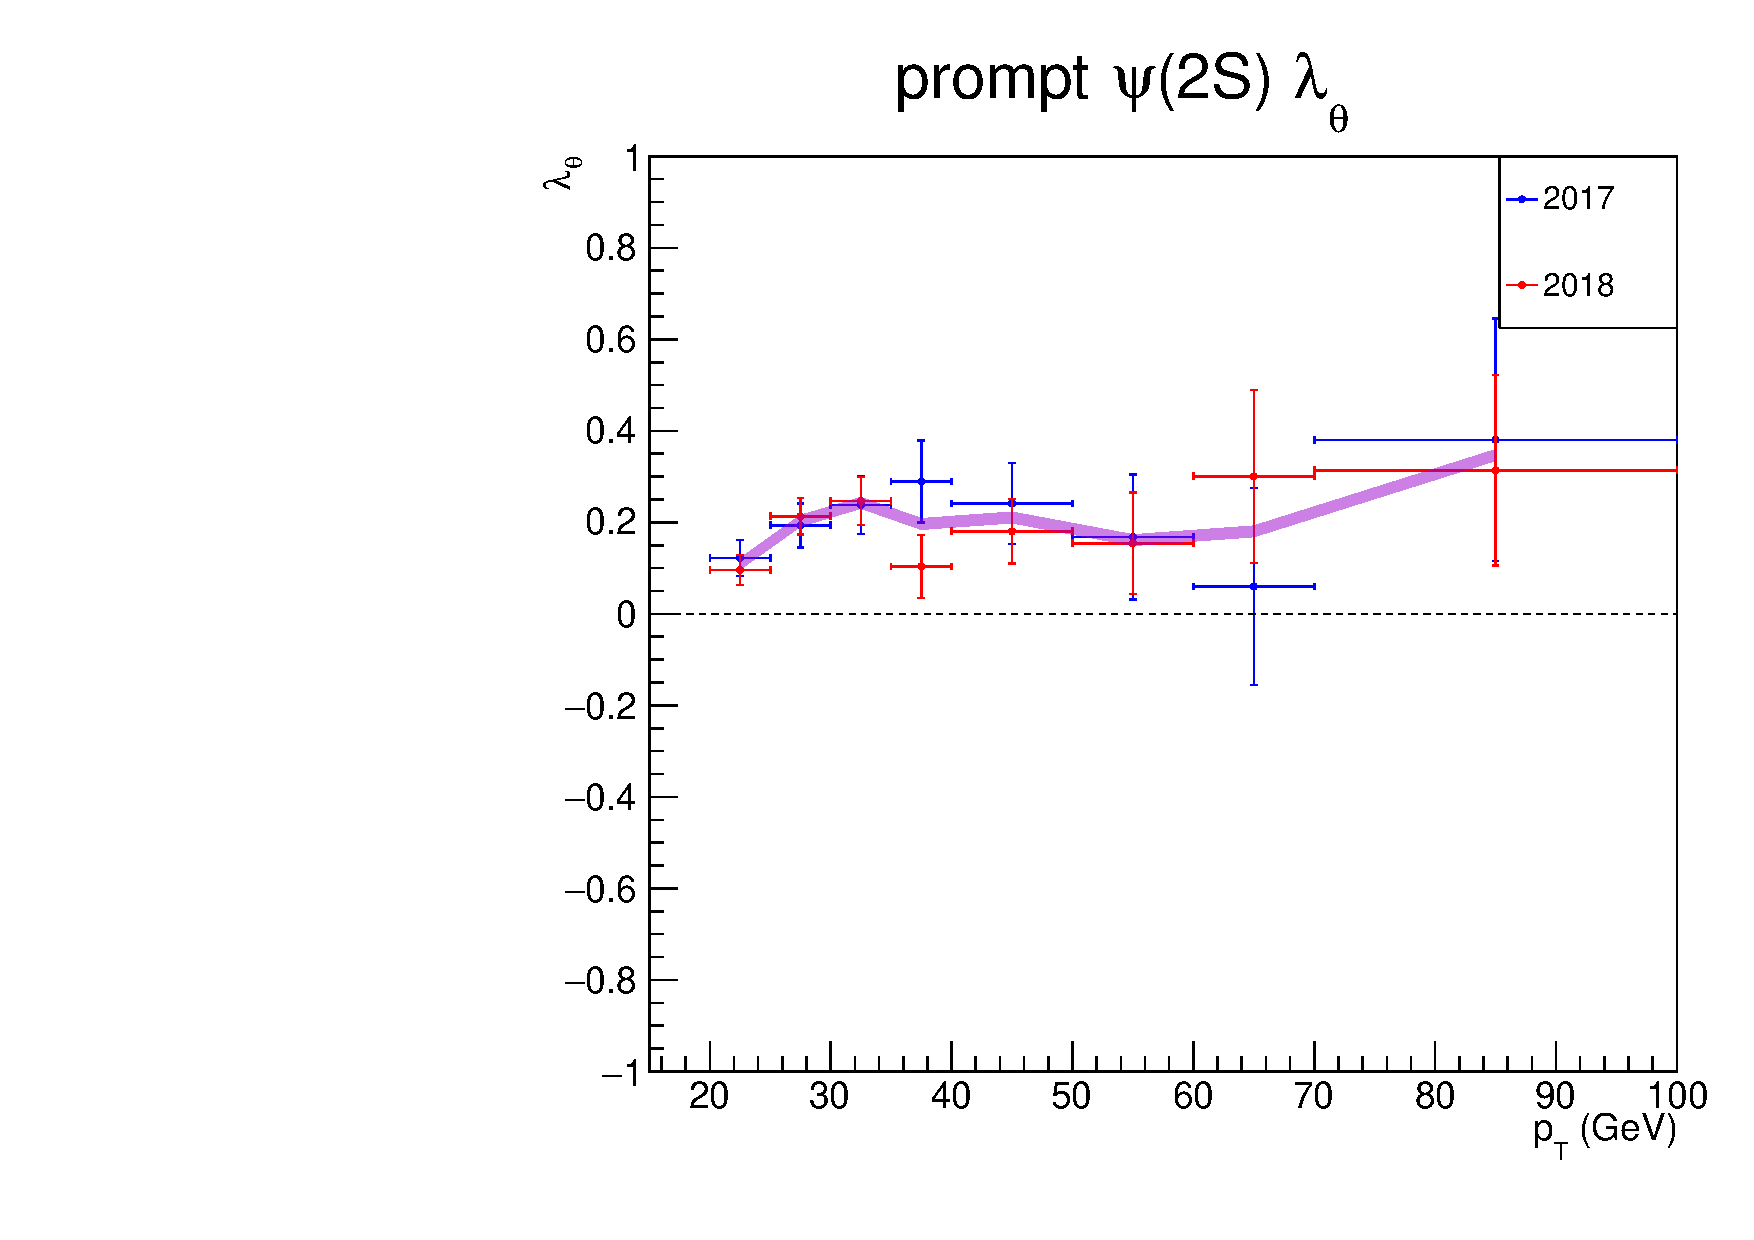
\includegraphics[width = 0.48\textwidth]{Figures/chapter6/par_lth_years_unc-psip.pdf}
\caption{\lth parameter fitted from each of the two years of data taking, 
for the \jpsi (left) and \psip (right) analyses.
The pink band represents a systematic uncertainty of $\pm 0.012$.}
\label{fig:2017vs2018}
\end{figure}

\vfill\newpage

\subsection{Fit model of the dimuon mass distributions}

The \jpsi line shape does not enter directly 
in the determination of the fraction of mass continuum muon pairs 
in the signal region, 3.0--3.2\GeV,
because we use, as denominator, the number of counted events.
Besides, the signal function 
(two Crystal-Ball functions plus one Gaussian function) 
has enough freedom to adapt to the measured data, 
without biasing the fit of the continuum background.
The same arguments apply, naturally, to the \psip analysis.

The biggest source of uncertainty comes from the fact that we impose 
an exponential function for the description of the continuum background.
To evaluate the potential impact of this choice we have redone the \lth
measurement replacing the exponential by a linear function.
The new results are virtually identical to the baseline values.
Therefore, no uncertainty is assigned to these effects.

It is worth noting that the low-mass edge of the LSB windows,
both for the \jpsi and \psip cases, 
were set to higher values than allowed by the trigger to avoid edge effects.

Figure~\ref{fig:mass-fit-syst} shows, for illustration, 
the variation of \lth for the \jpsi and \psip analyses, 
when the mass continuum background is fitted with a linear function, 
with respect to the baselines values.

\begin{figure}[h]
\centering
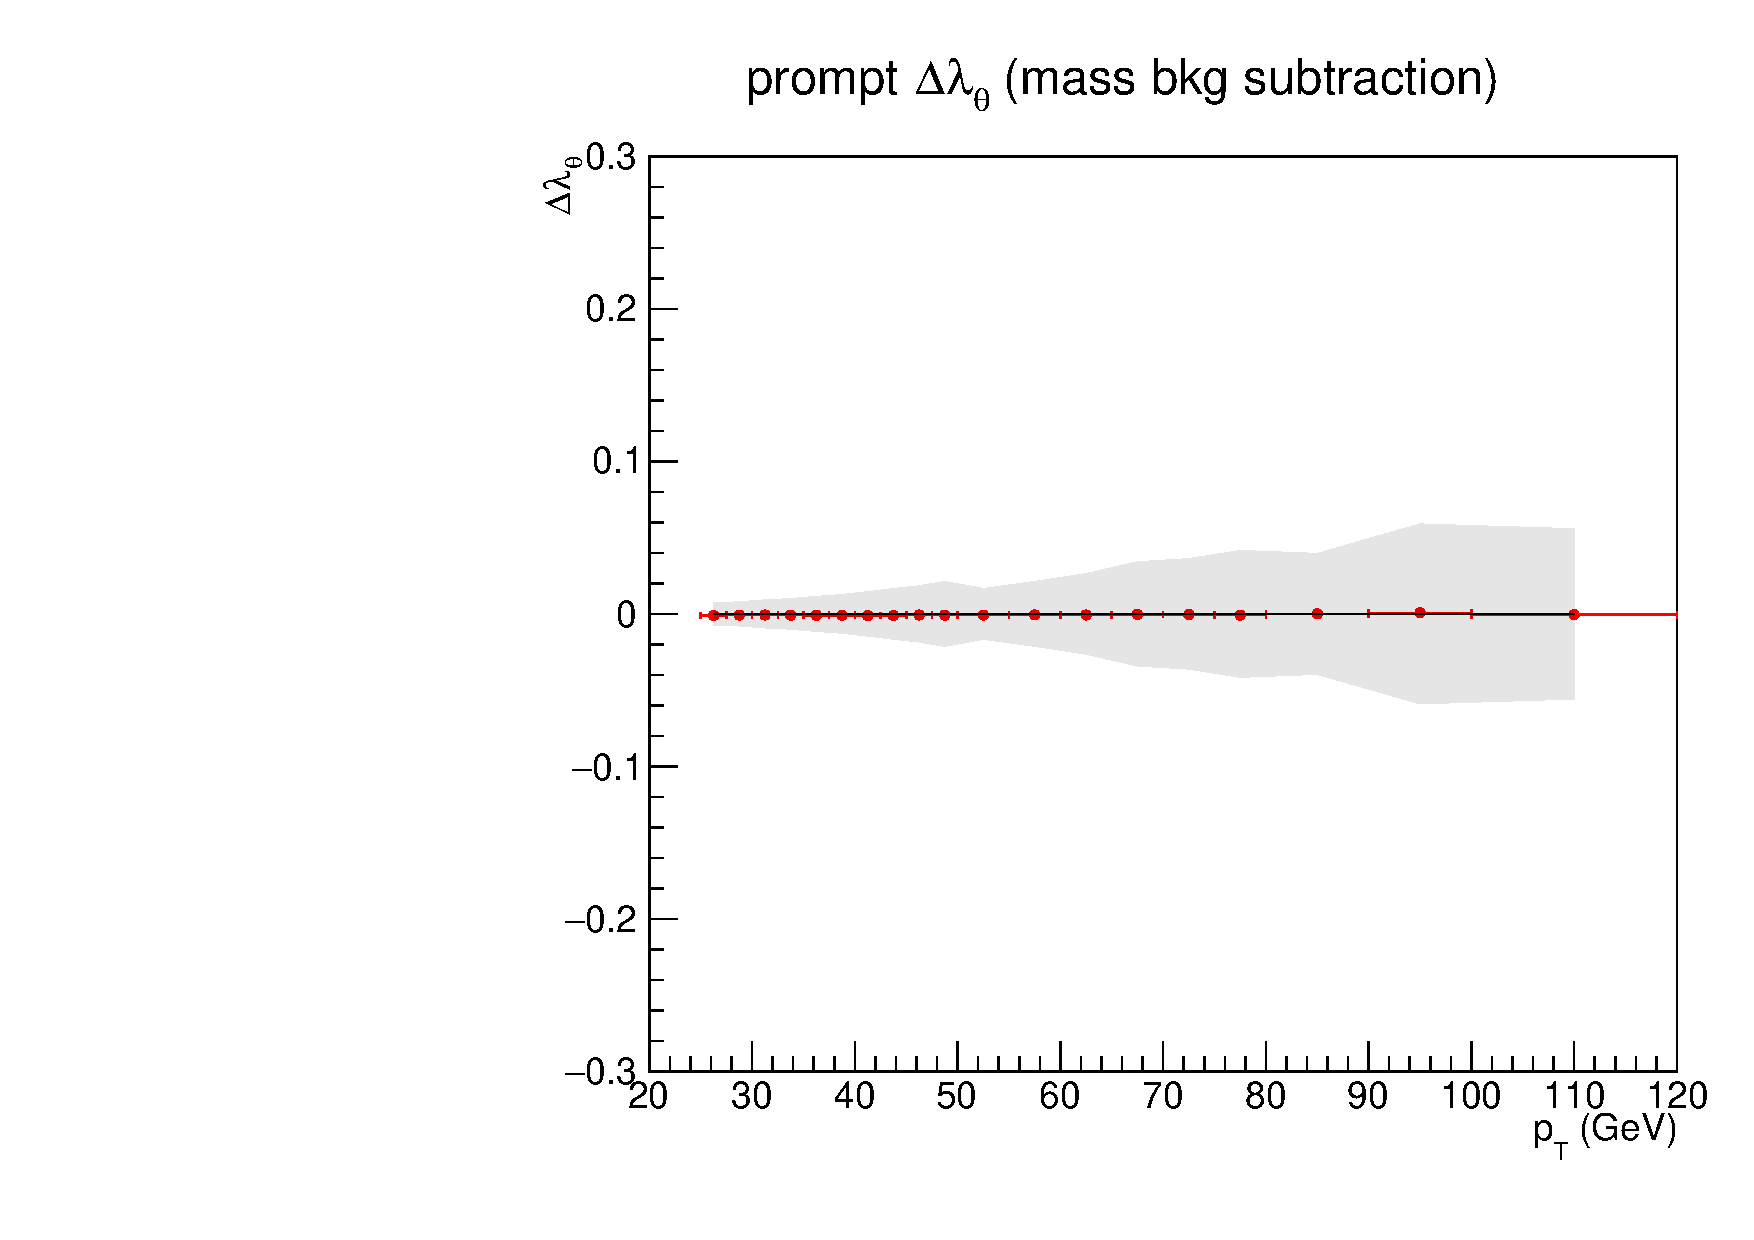
\includegraphics[width = 0.48\textwidth]{Figures/chapter6/lth_absDiff_M-jpsi.pdf}
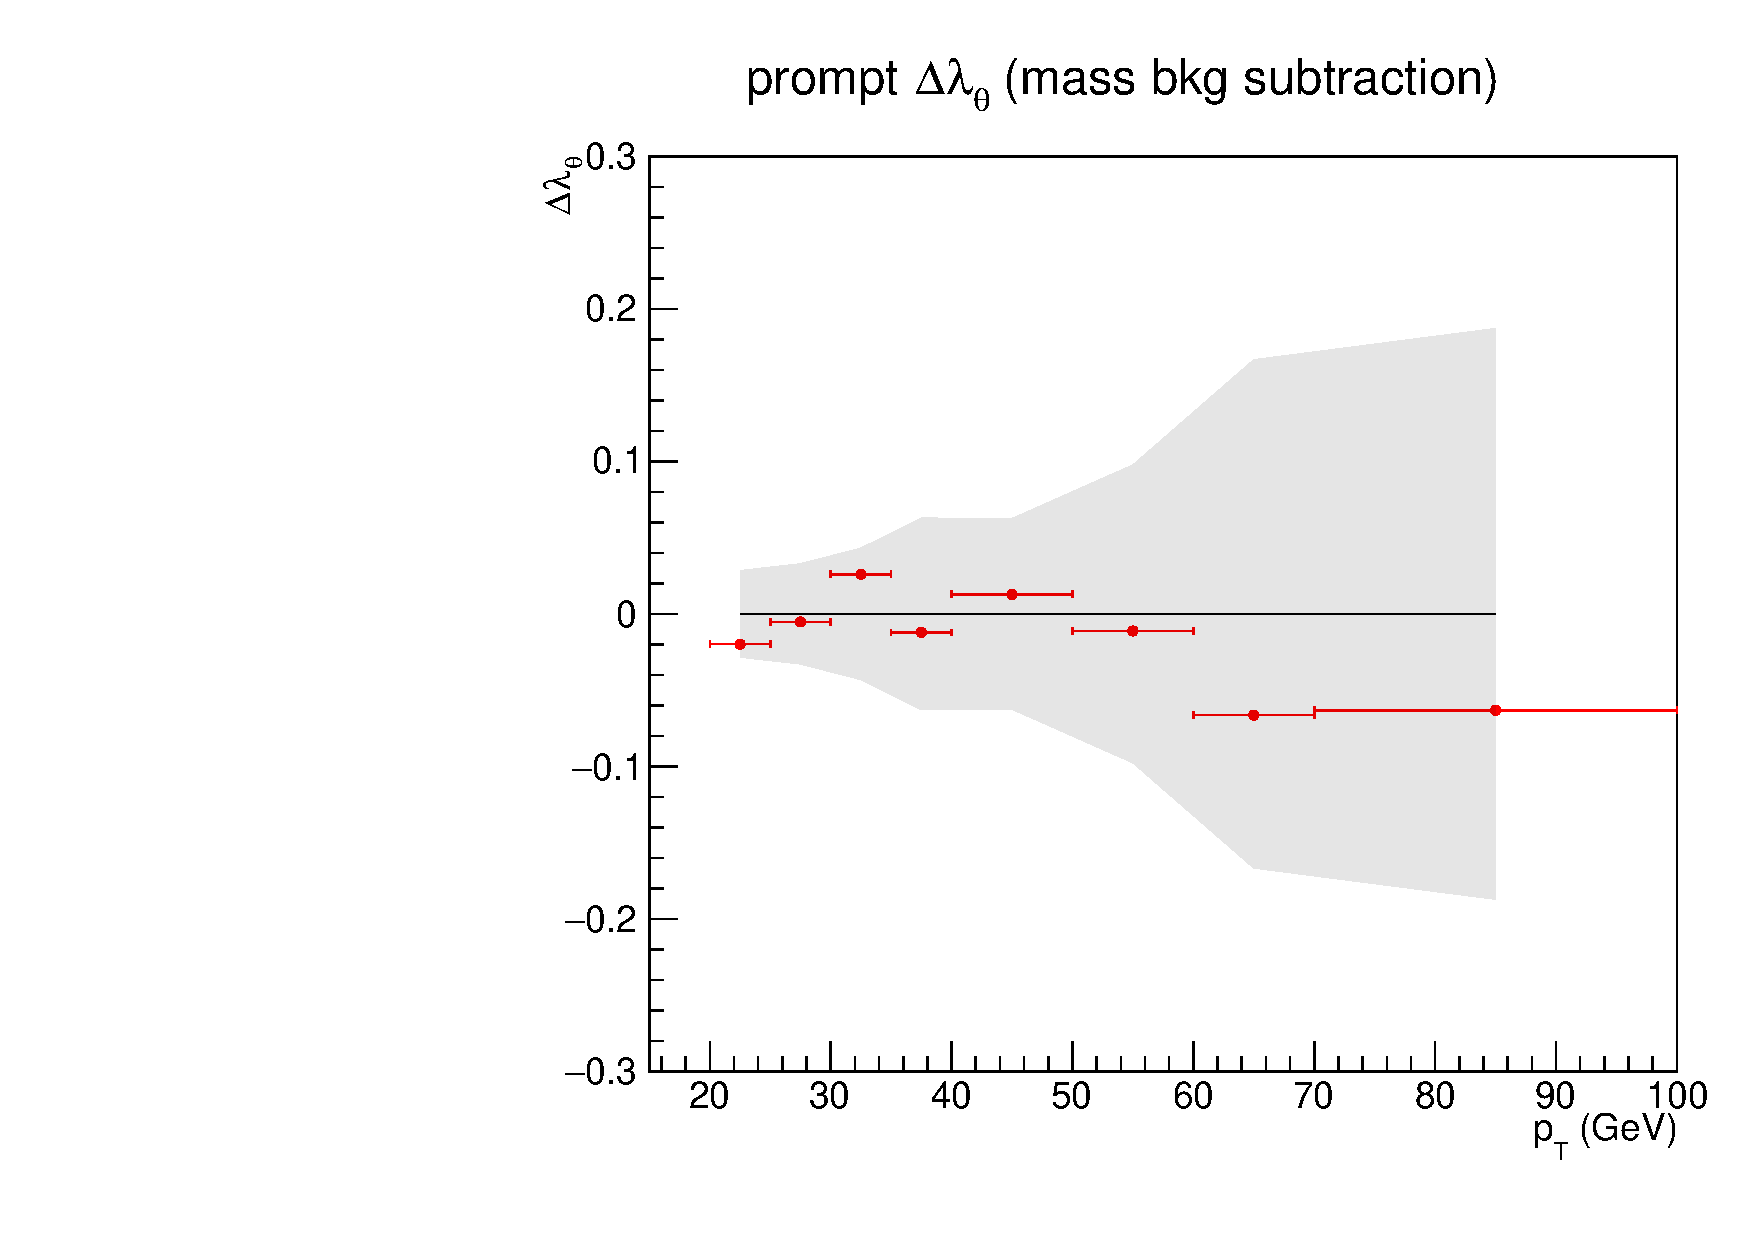
\includegraphics[width = 0.48\textwidth]{Figures/chapter6/lth_absDiff_M-psip.pdf}
\caption{Differences between the \lth values obtained with the varied 
dimuon mass fit model and the baseline procedure, 
compared to the statistical uncertainties of the baseline measurement (grey band),
for the \jpsi (left) and \psip (right) analyses.}
\label{fig:mass-fit-syst}
\end{figure}

\vfill\newpage

\subsection{Single muon detection efficiencies}

The single muon \pt cut of 5.6\GeV ensures that 
all the selected events have muons of similar detection efficiencies (in the plateau),
so that an inaccurate parametrization of the efficiency curve will have 
a negligible impact on the results.
For the muons in the region $|\eta| < 0.2$, however, 
the ``turn-on region" is not completely removed,
as can be seen in Fig.~\ref{fig:single_mu_eff_syst1}.

\begin{figure}[h]
\centering
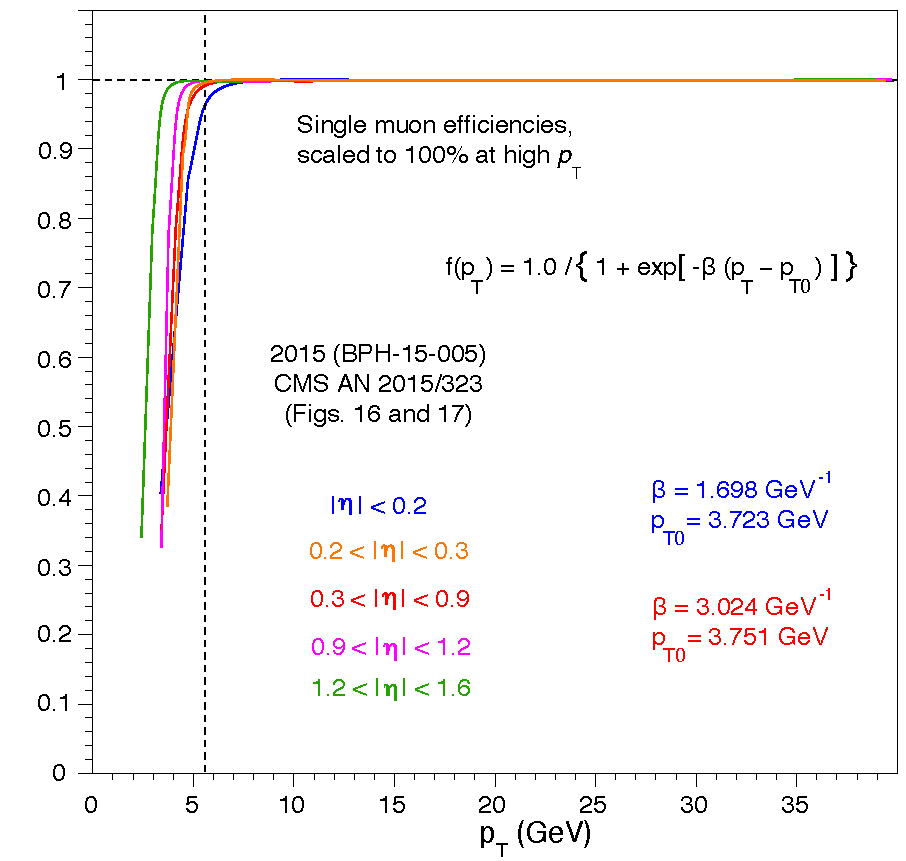
\includegraphics[width=0.55\textwidth]{Figures/chapter6/single_mu_effs_2015.pdf}
\caption{Single muon detection efficiencies for muons in several exclusive 
$\abs{\eta}$ bins, as used in the BPH-15-005 cross section measurements.}
\label{fig:single_mu_eff_syst1}
\end{figure}

We considered two checks to evaluate if the results might be affected 
by a potentially wrong efficiency correction of the events in this $\eta$ region.
\begin{itemize}
\item \textbf{Efficiency curve reweighing}:\\
We take the single muon efficiency function for this $\eta$ range,
$$f(\pt) = \frac{1}{1+\exp\left[-\beta \cdot \left(\pt-{\pt}_0 \right) \right]}
\hspace{0.9cm}(\beta=1.698,\hspace{0.2cm}{\pt}_0=3.723)$$
and consider two extreme cases: 
\begin{enumerate}
\item[1)] There is no inefficiency at all: we weigh the MC events by $1/f(\pt)$;
\item[2)] The real efficiency differs from the MC efficiency by an amount equal to the efficiency itself: 
we weigh the MC events by $f(\pt)$.
\end{enumerate} 
\item \textbf{\pt cut}:\\ 
We increase the \pt cut from 5.6 to 6.7\GeV for the muons with $|\eta| < 0.2$, 
completely removing their turn-on region.
\end{itemize} 

%\vfill\newpage

The differences between the \lth values obtained in each of these three alternative analyses 
and those of the baseline analysis are shown in Fig.~\ref{fig:single_mu_eff_syst2},
for the \jpsi (left) and \psip (right) analyses,
together with a grey band centred at zero that represents 
the statistical uncertainty of the baseline results.

We assign a systematic uncertainty from this source, 
up to 50\GeV for the \jpsi and up to 40\GeV for the \psip, 
computed (conservatively) as the average of the absolute differences between 
each of the two reweighing options and the baseline values.

\begin{figure}[h]
\centering
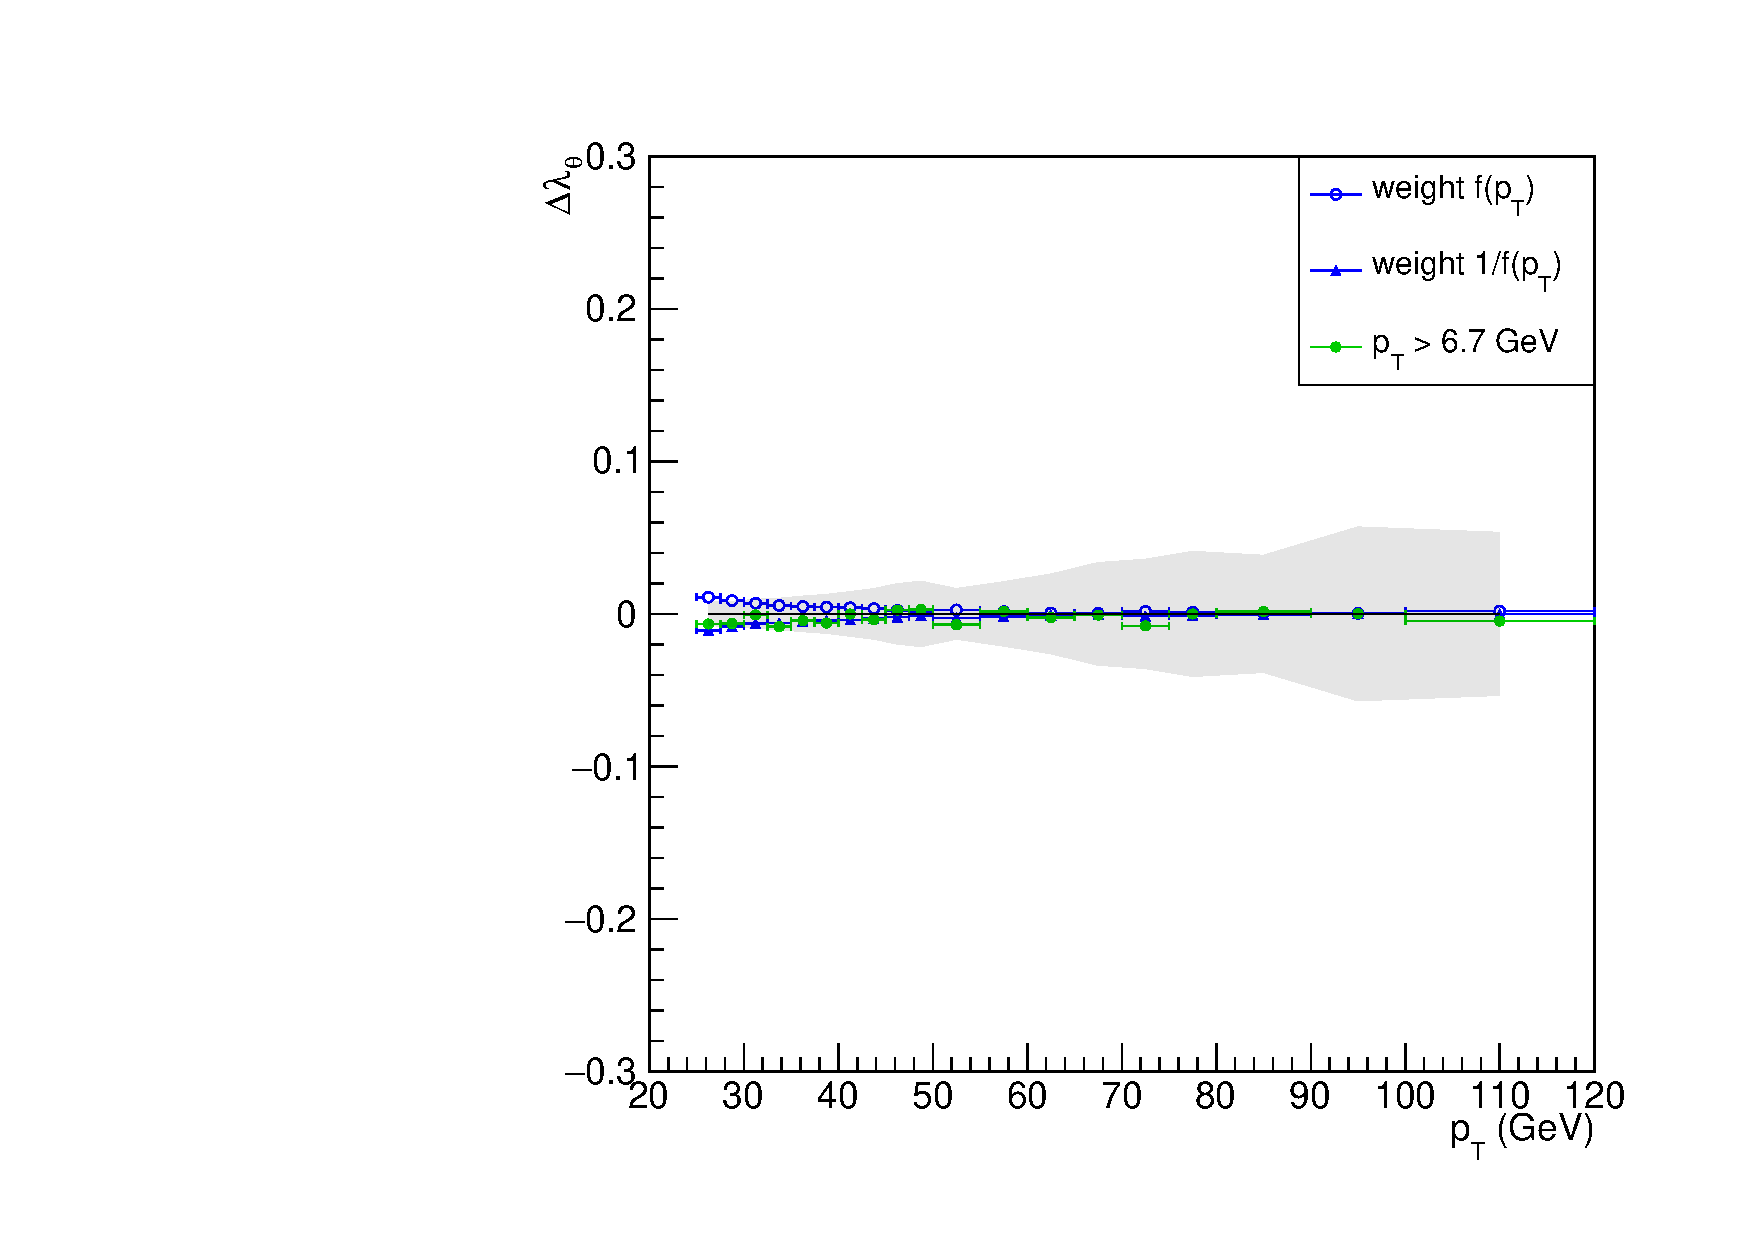
\includegraphics[width=0.43\textwidth]{Figures/chapter6/lth_absDiff_muEff-jpsi.pdf}
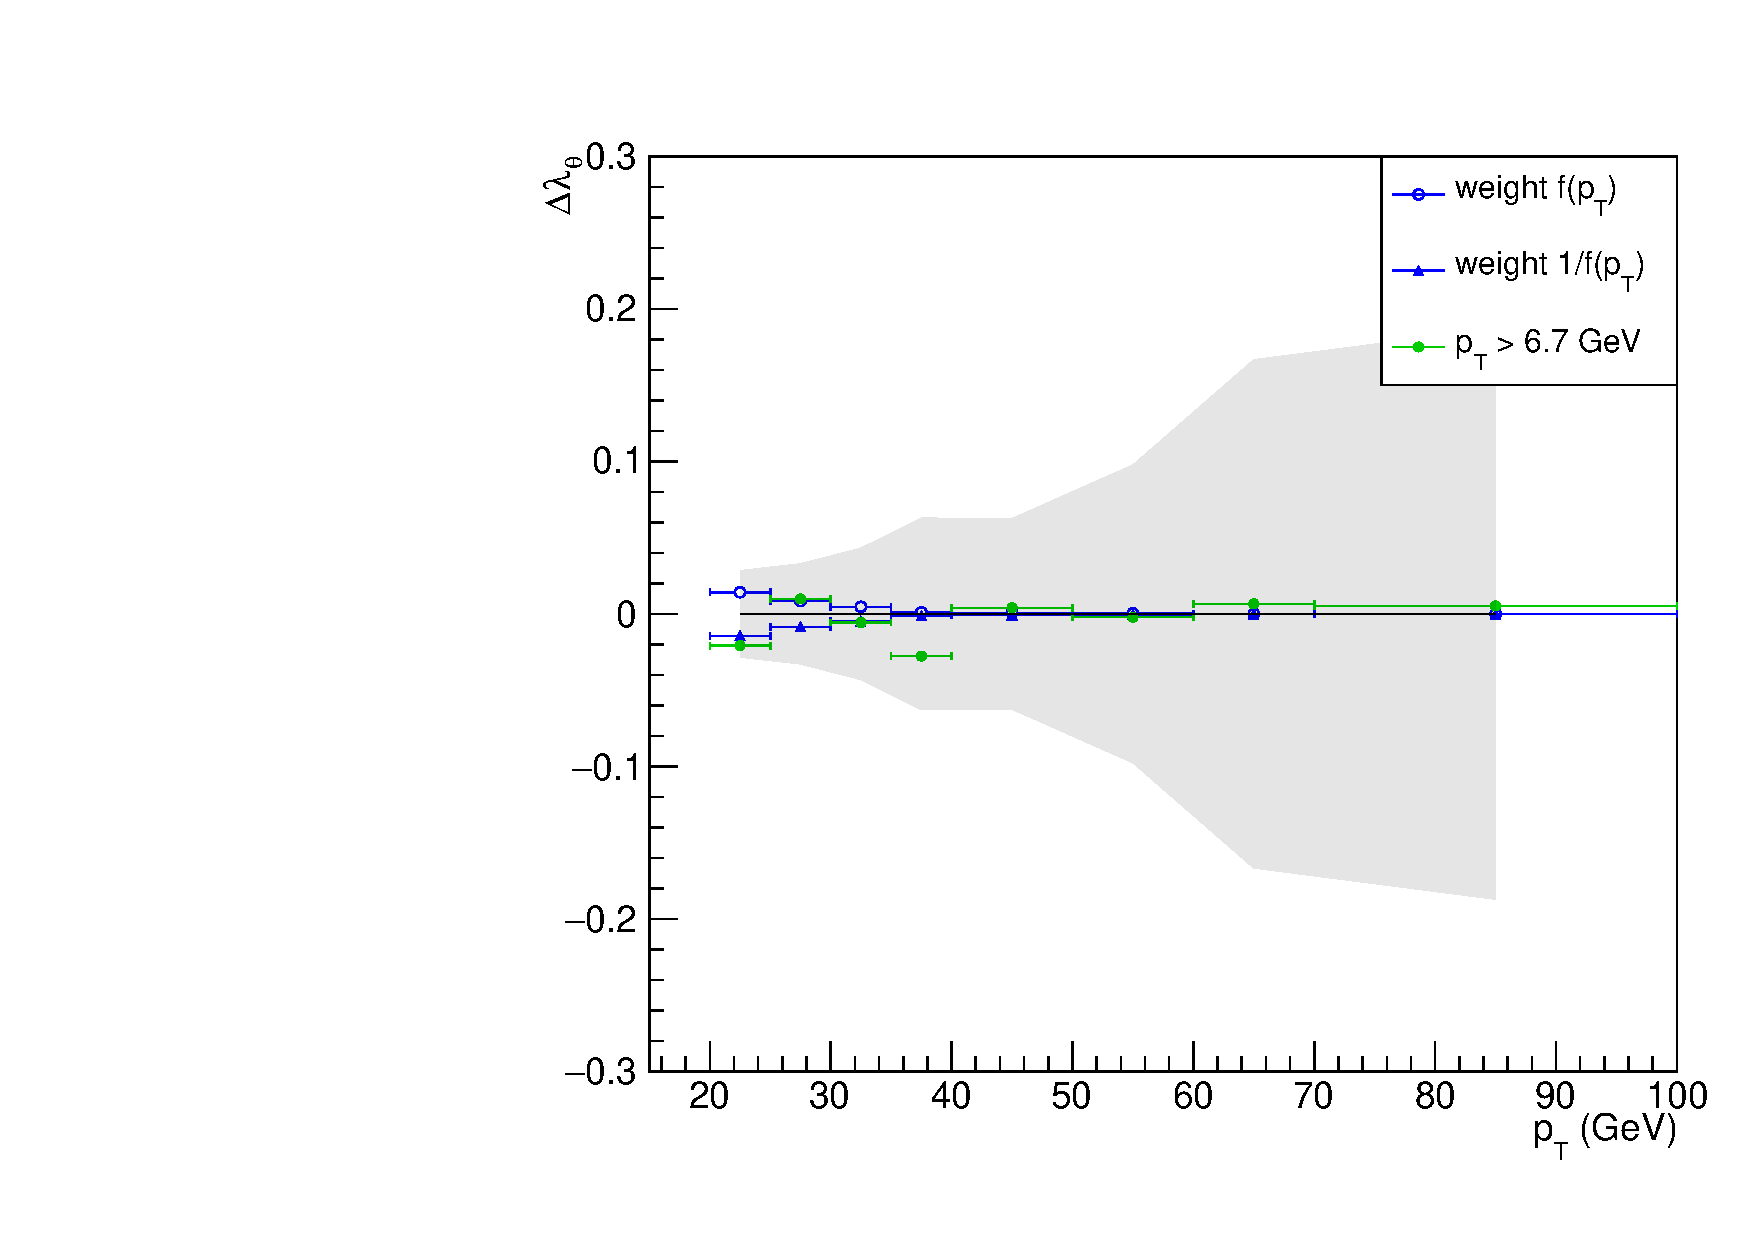
\includegraphics[width=0.47\textwidth]{Figures/chapter6/lth_absDiff_muEff-psip.pdf}
\caption{Differences between the \lth values obtained in each of the three alternative
analysis scenarios and the baseline procedure, compared to the statistical uncertainties
of the baseline measurement (grey band), for the \jpsi (left) and \psip (right) analyses.}
\label{fig:single_mu_eff_syst2}
\end{figure}

The muons produced with pseudorapidity in the $0.2 < |\eta| < 0.3$ region 
have a lower muon detection efficiency because of the gap between the central wheel 
and its neighbours.
To evaluate the possible impact of a miscorrection of this efficiency,
we measured \lth after rejecting all events with a muon (or both) in this $\eta$ region.
As shown in Fig.~\ref{fig:single_mu_eff_eta} for the \jpsi and \psip analyses,
the difference between the varied and baseline \lth values, vs.\ \pt,
is randomly distributed around zero; the deviations seem to be purely statistical.
Therefore, we do not assign a systematic uncertainty to this source.

\begin{figure}[h]
\centering
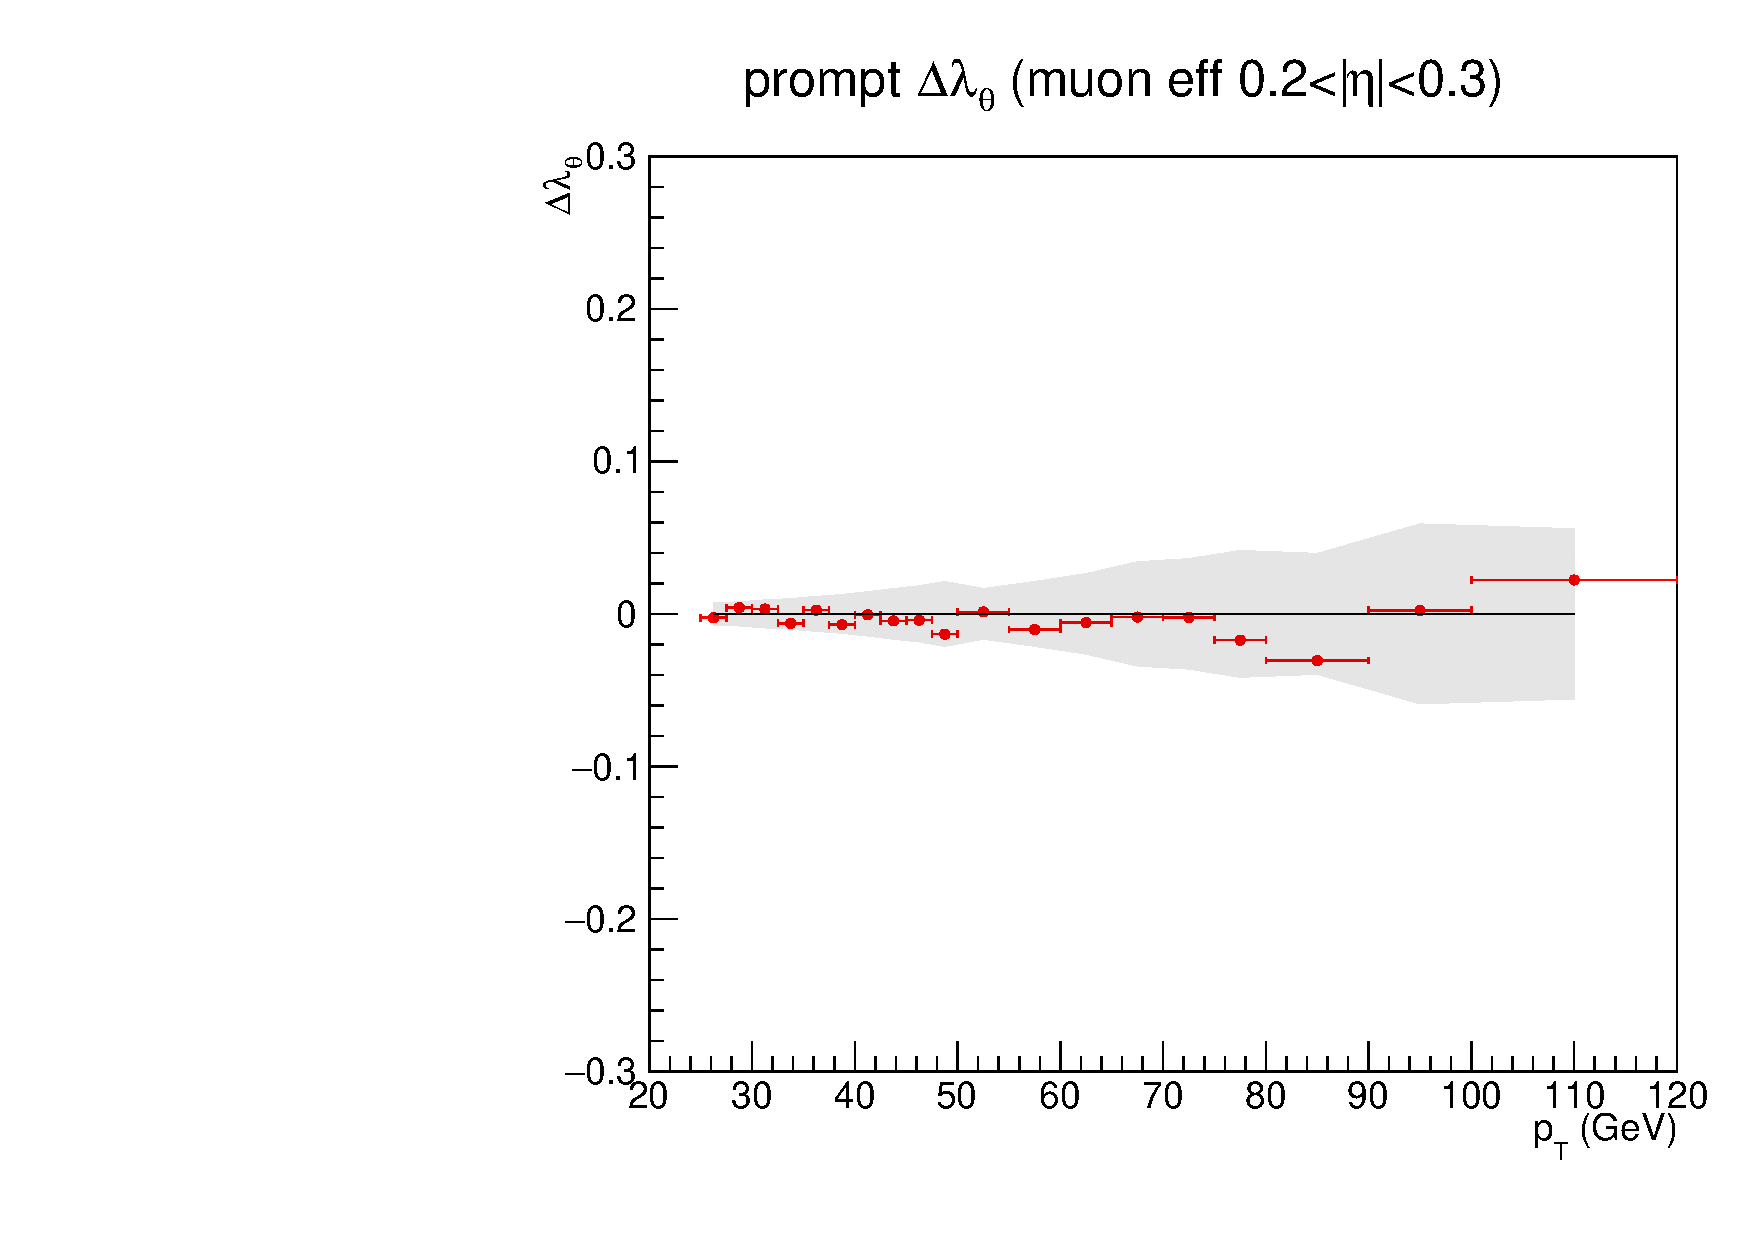
\includegraphics[width=0.45\textwidth]{Figures/chapter6/lth_absDiff_eta-jpsi.pdf}
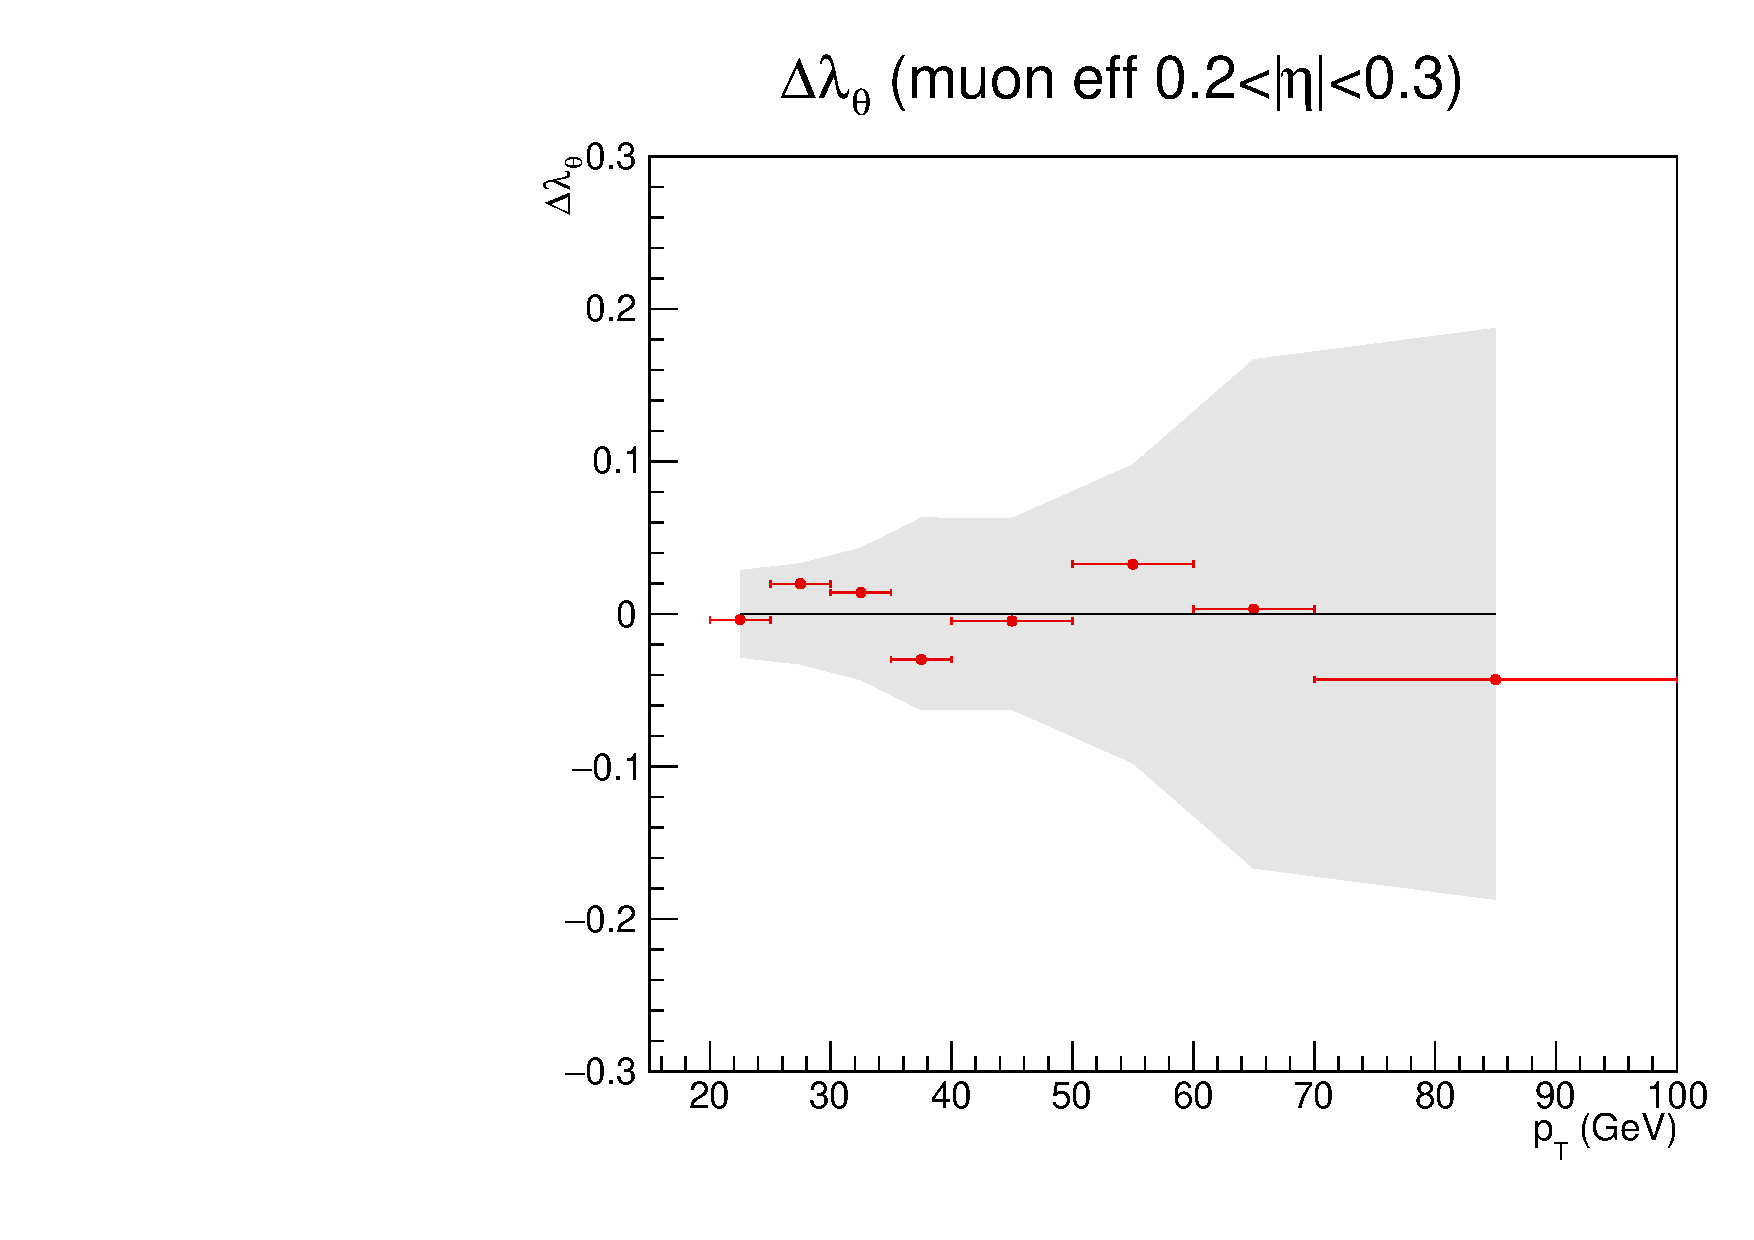
\includegraphics[width=0.45\textwidth]{Figures/chapter6/lth_absDiff_eta-psip.pdf}
\caption{Differences between the \lth values obtained when rejecting events with
at least one muon in the $0.2 < |\eta| < 0.3$ region and the baseline procedure, 
compared to the statistical uncertainties of the baseline measurement (grey band), 
for the \jpsi (left) and \psip (right) analyses.}
\label{fig:single_mu_eff_eta}
\end{figure}

\vfill\newpage

\subsection{Dimuon detection efficiencies (``$\rho$ factor")}

The dimuon efficiency is smaller than the product of the two single muon efficiencies, 
due to trigger-induced muon-pair correlations that become significant at high \pt:

\begin{equation}
\epsilon_{\mu\mu}=\epsilon_{\mu,1}\cdot\epsilon_{\mu,2}\cdot\rho \, .
\end{equation}

In principle, this effect should be faithfully reproduced by the detailed trigger emulation,
included in the MC simulation, but it is important to evaluate if our results could be affected
by some residual differences.
%
Our study follows exactly the same procedure as used in the BPH-13-003 analysis
(``Measurement of the prompt \jpsi and \psip polarizations in pp collisions at $\sqrt{s} = 7$\TeV");
all the details are explained in detail in the 
\href{https://cms.cern.ch/iCMS/jsp/db_notes/noteInfo.jsp?cmsnoteid=CMS\%20AN-2013/016}{\textcolor{blue}{analysis note AN-13-016}}.

The dimuon trigger efficiency is studied by comparing the MC event distributions 
obtained after applying the trigger (``trig") to those obtained before (``reco").
We restrict our study to $\pt > 50$\GeV events, where the effects are more visible.
%
As can be seen in Fig.~\ref{fig:DeltaR},
the trig/reco ratio of the $\Delta\phi$ vs.\ $\Delta\eta$ 2D distribution 
shows that the trigger efficiency is very low when the two muons are 
``too close to each other" in the variable $\Delta R = \sqrt{\Delta\phi^2 + \Delta\eta^2}$.

\begin{figure}[h]
\centering
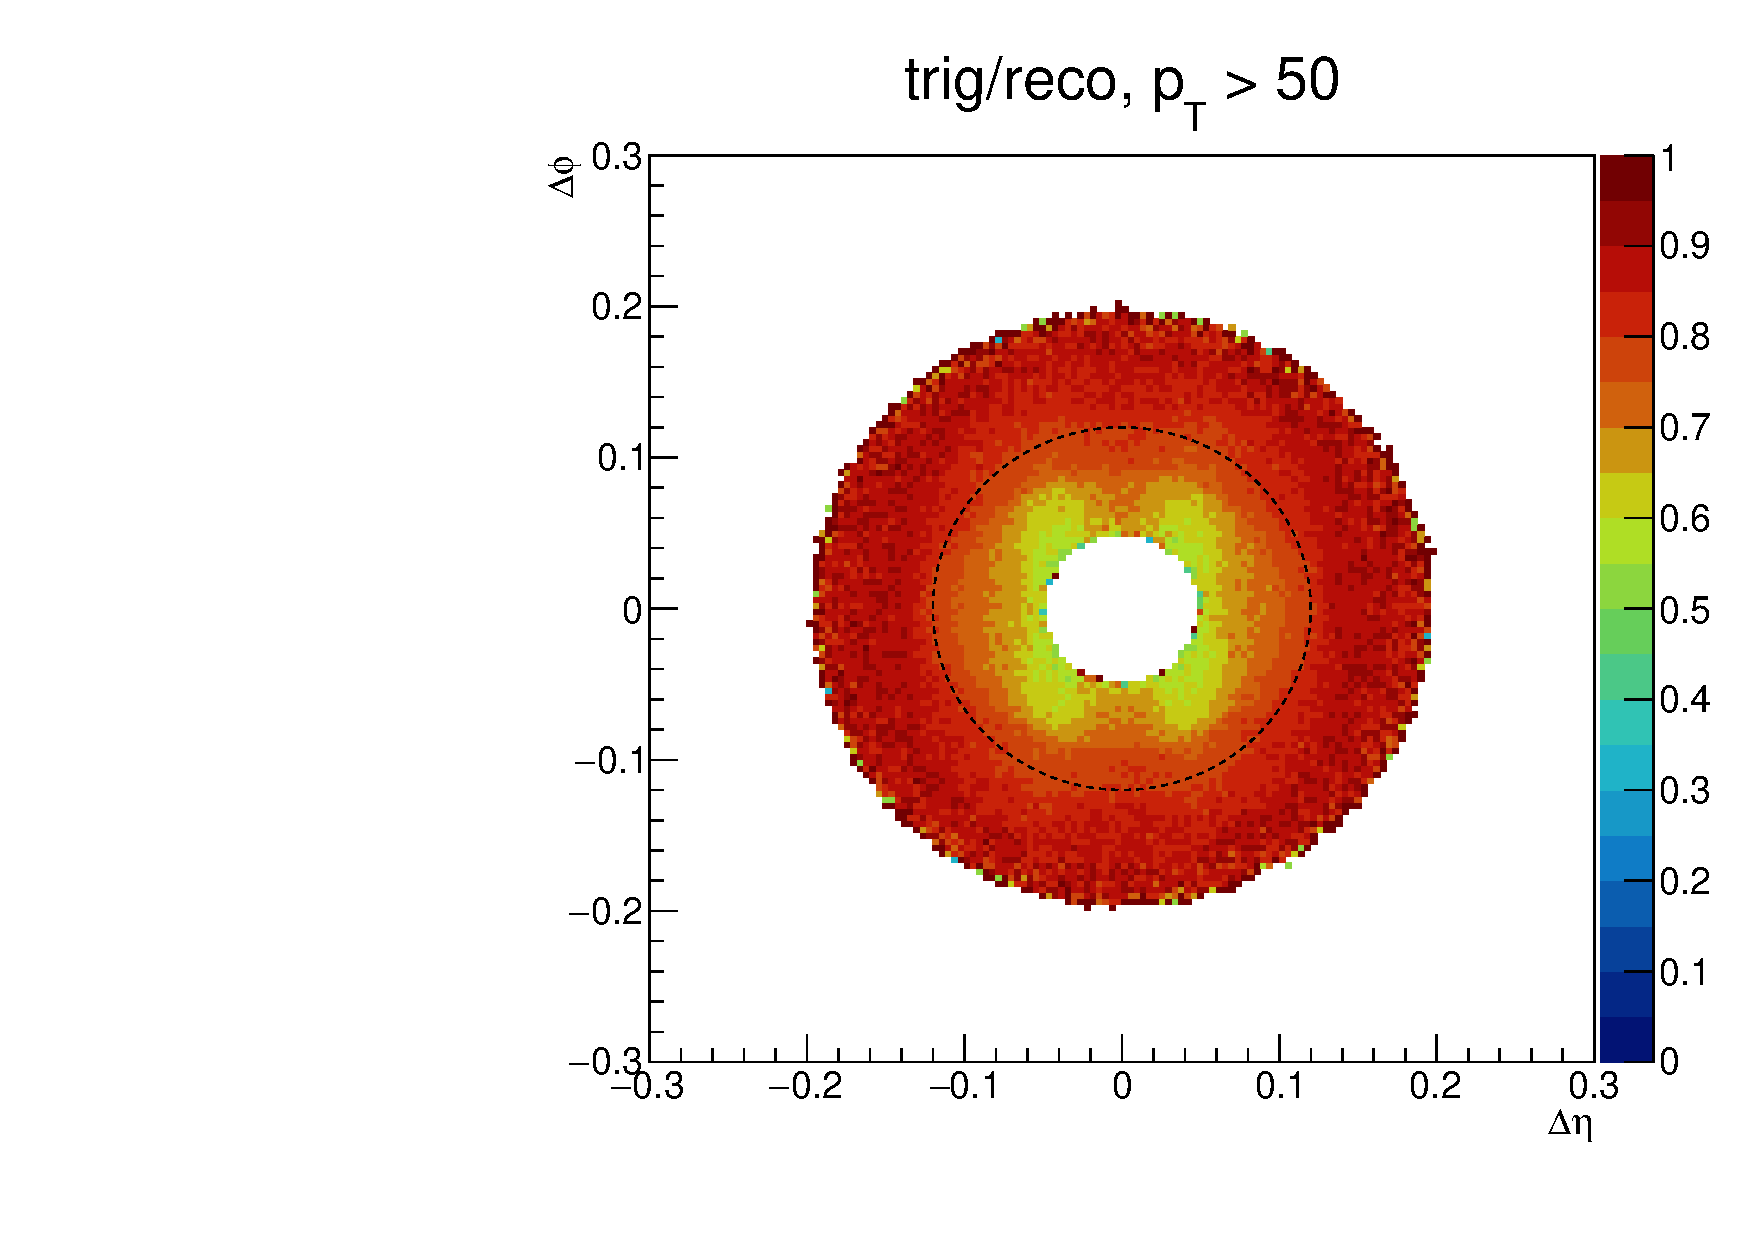
\includegraphics[width=0.45\textwidth]{Figures/chapter6/AEtaPhi_full.pdf}
\caption{Ratio between simulated 2D event distributions,
after over before applying the trigger emulation, 
for \jpsi dimuons of $\pt > 50$\GeV, 
in the $\Delta\phi$ vs.\ $\Delta\eta$ plane.}
\label{fig:DeltaR}
\end{figure}

\begin{figure}[ht]
\centering
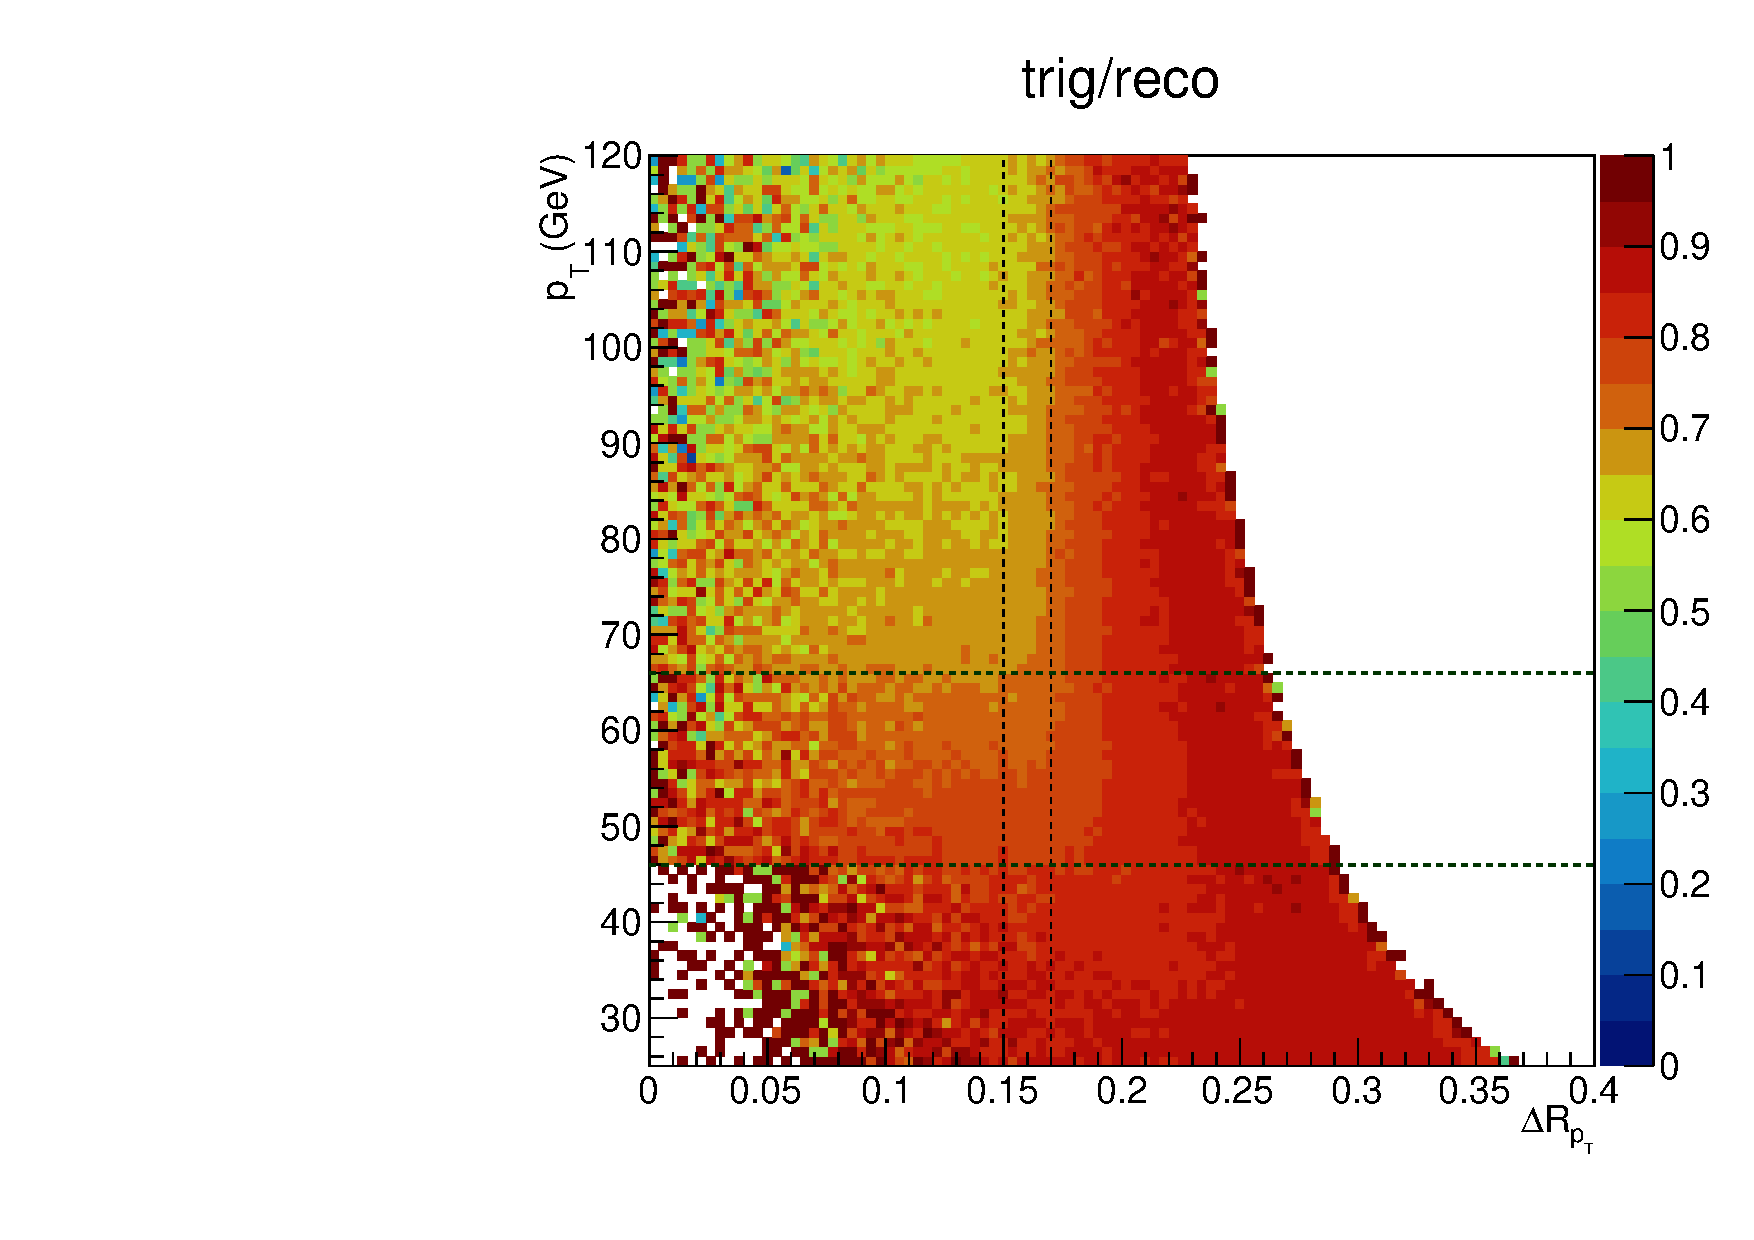
\includegraphics[width=0.45\textwidth]{Figures/chapter6/RpTpT.pdf}
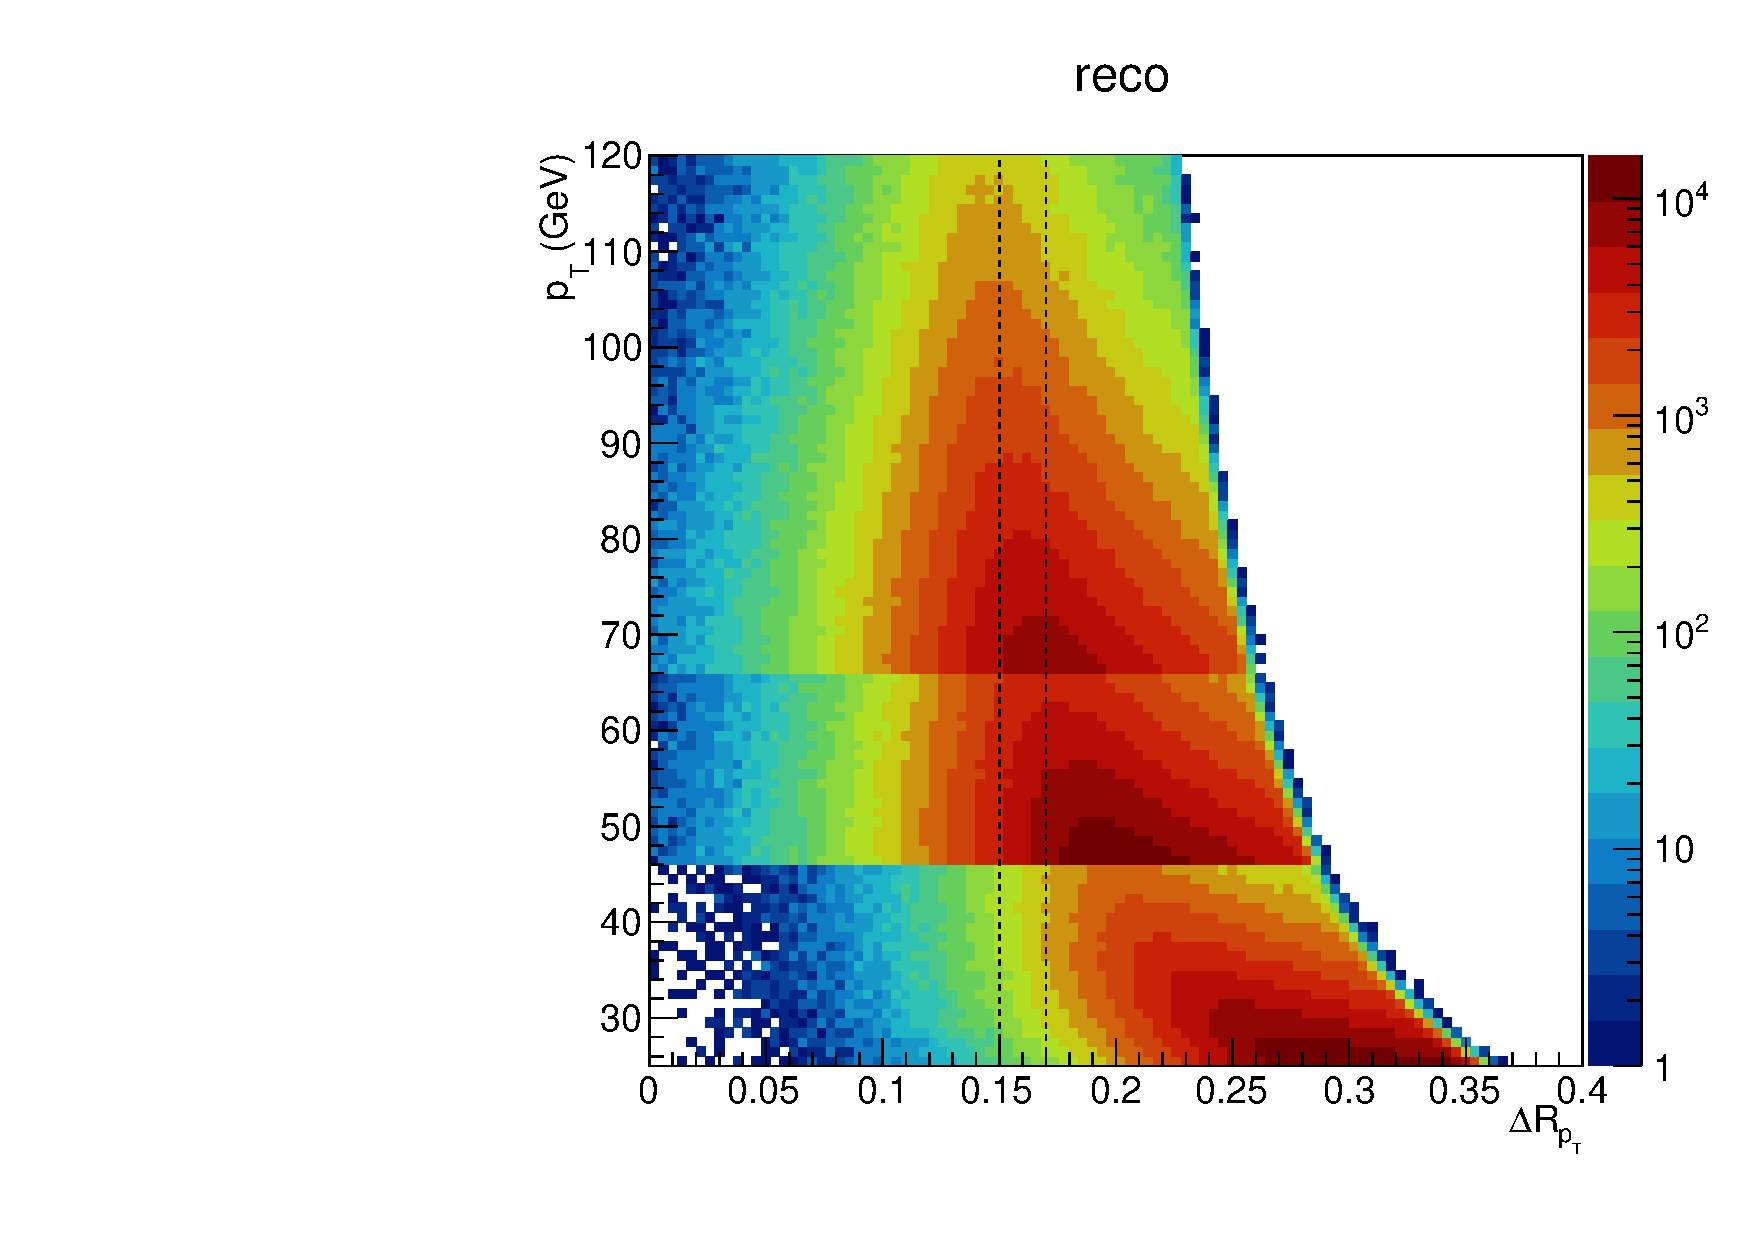
\includegraphics[width=0.45\textwidth]{Figures/chapter6/RpTpT_r.pdf}
\caption{Left: Ratio between simulated 2D event distributions,
after over before applying the trigger emulation, 
for \jpsi dimuons of $\pt > 50$\GeV, 
in the \pt vs.\ $\Delta R_{\pt}$ plane.
Right: Corresponding event distribution before applying the trigger emulation.}
\label{fig:DeltaRpT}
\end{figure}

The dimuon trigger efficiency depends also on the difference between the \pt of the two muons, 
$\Delta \pt$, and it is easier to isolate and reject regions of low dimuon efficiency if 
we apply cuts on the variable $\Delta R_{\pt}$, defined as

\begin{equation}
\Delta R_{\pt} = \sqrt{\Delta\phi^2+\Delta\eta^2}+\frac{\log|\Delta\pt|}{b}\hspace{0.9cm}(b=45) \, .
\end{equation}


Figure~\ref{fig:DeltaRpT}-left shows that rejecting events of $\Delta R_{\pt} < 0.17$
leads to a \jpsi event sample where all the dimuons have trigger efficiency above 70\%,
so that we are much less sensitive to the accuracy of the MC efficiency correction.
%
Figure~\ref{fig:DeltaRpT}-right shows the \pt vs.\ $\Delta R_{\pt}$ 2D event distribution 
before applying the trigger emulation (the denominator of the ratio shown on the left panel).
We can see that a $\Delta R_{\pt} < 0.17$ cut rejects a very large fraction of the high-\pt events.
Therefore, for $\pt > 70$\GeV we use a looser cut, $\Delta R_{\pt} = 0.15$ 
(corresponding to an efficiency threshold of 60\%), 
to avoid losing too many events 
(otherwise the \lth measurement becomes too uncertain to provide meaningful results).

Since the $\Delta R_{\pt}$ cuts reduce the $\abscosth$ coverage,
we also recompute the baseline \lth fitting the $\abscosth$ distribution in the same range, 
to ensure that potential variations are exclusively caused by the $\rho$ factor.

\begin{figure}[h]
\centering
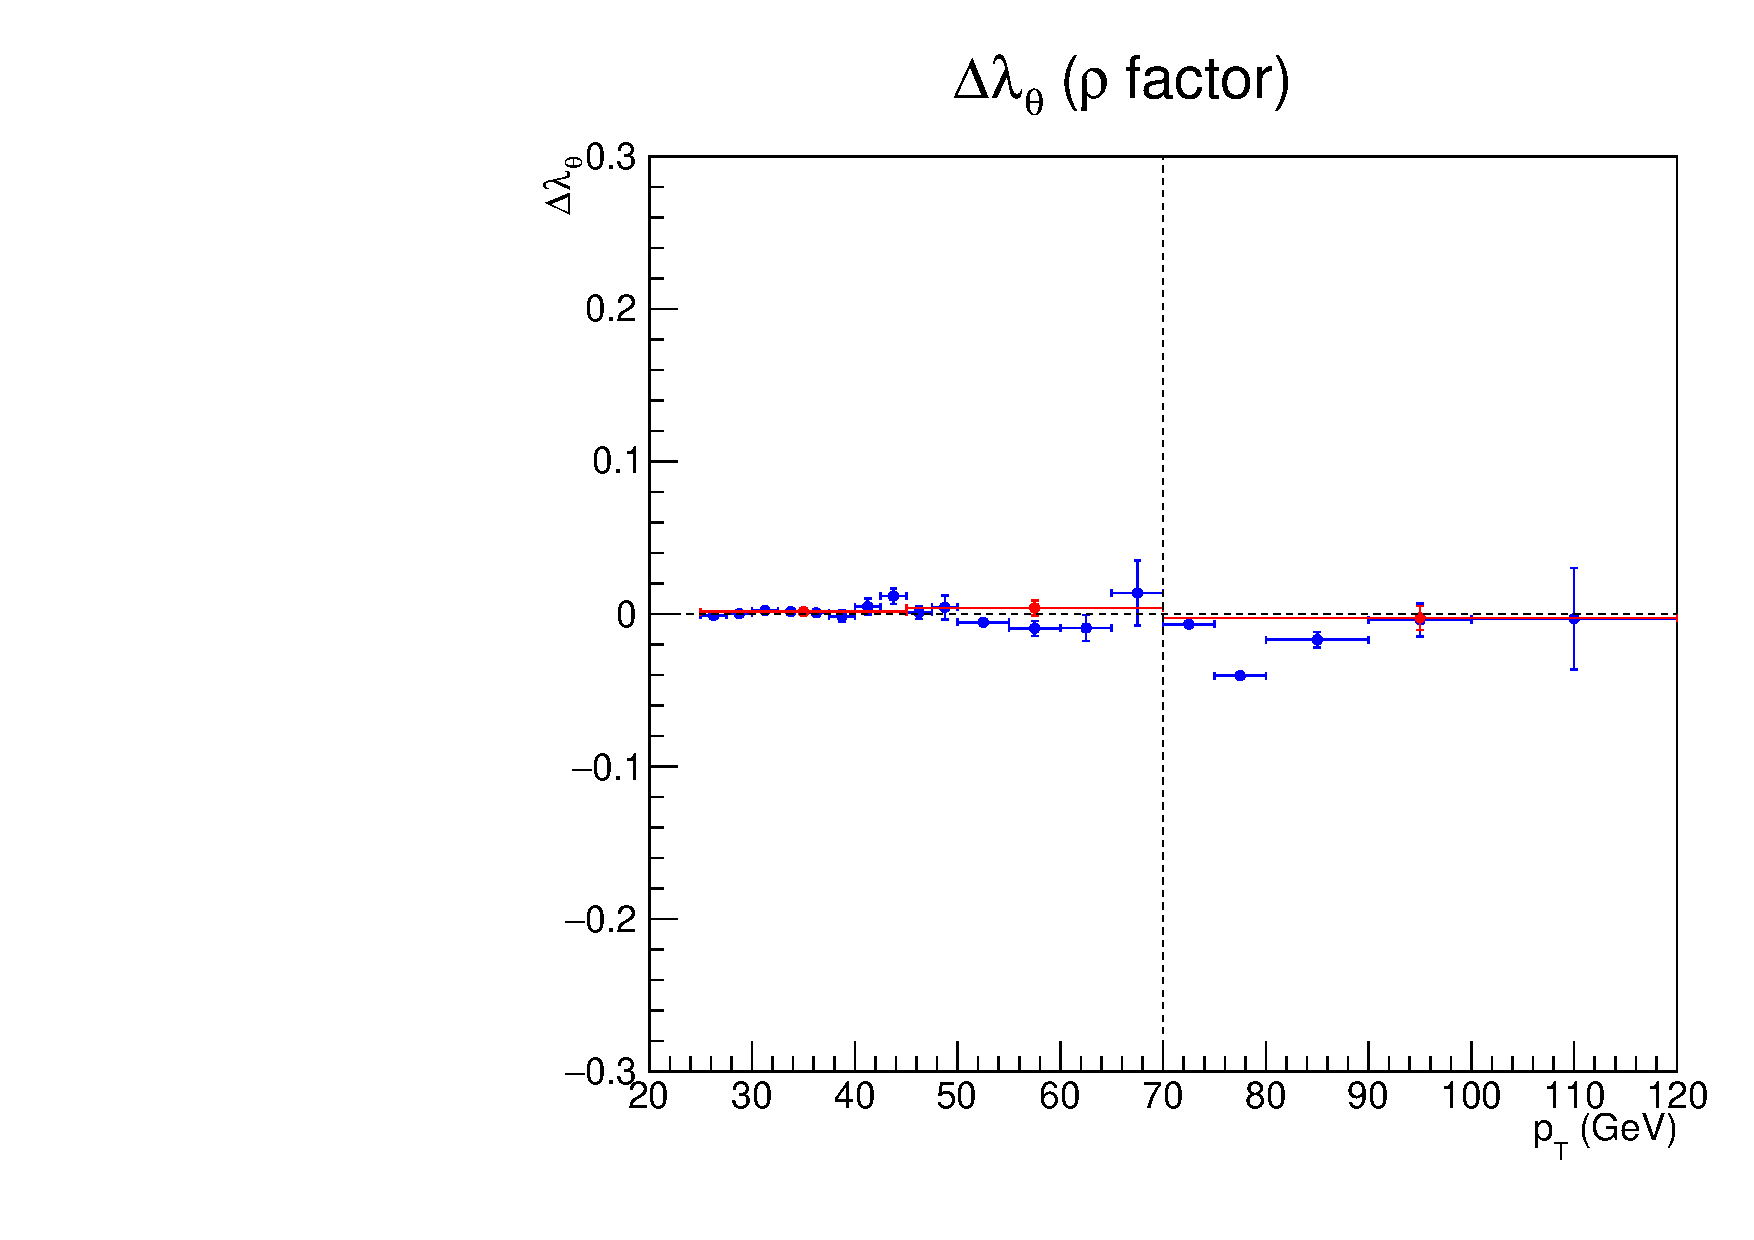
\includegraphics[width=0.48\textwidth]{Figures/chapter6/lth_absDiff_rho-jpsi.pdf}
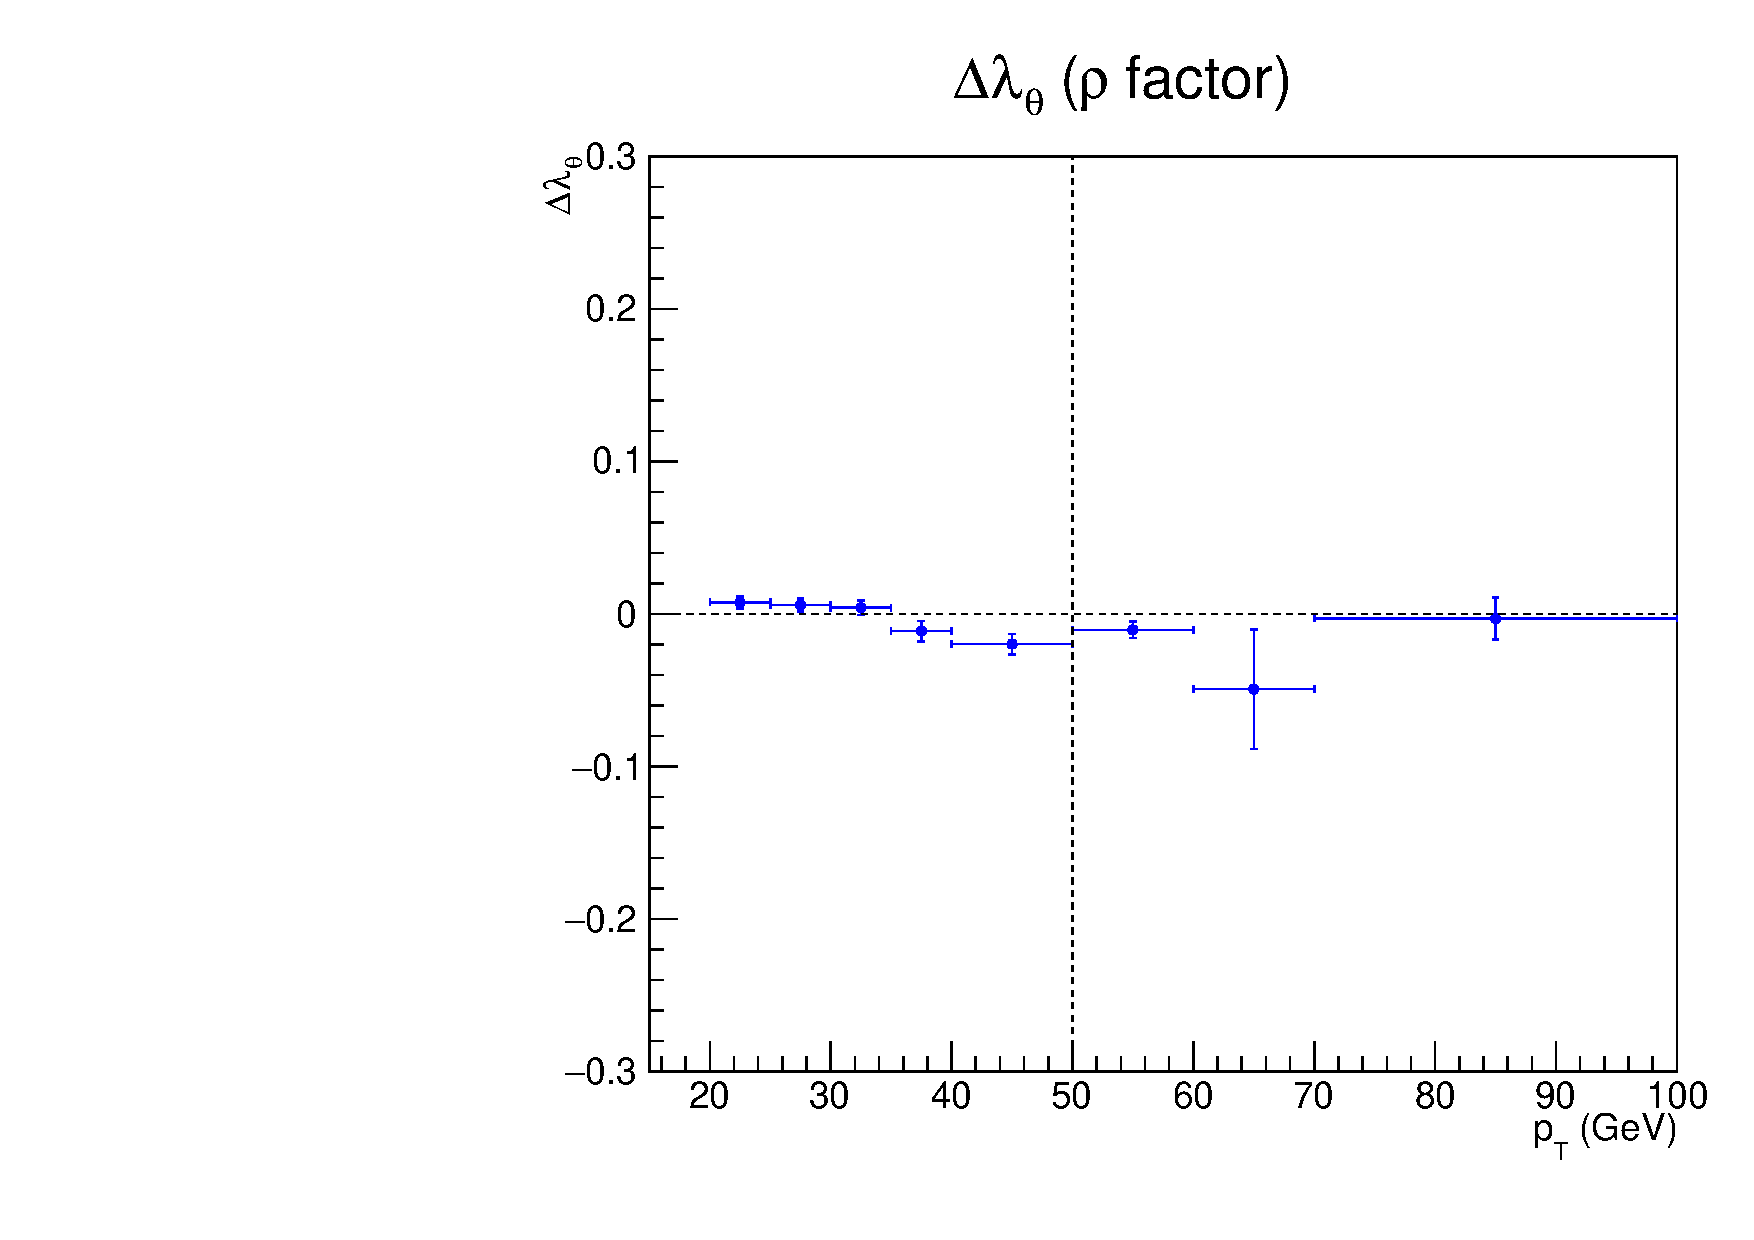
\includegraphics[width=0.48\textwidth]{Figures/chapter6/lth_absDiff_rho-psip.pdf}
\caption{Difference between the \lth values measured with and without
applying the $\Delta R_{\pt}$ cuts, vs.\ \pt, for the \jpsi (left) and \psip (right) analyses.}
%in the standard 19 \pt bins (blue points) and in a coarser \pt binning (red points).}
\label{fig:lth_absDiff_rho}
\end{figure}

Figure~\ref{fig:lth_absDiff_rho} shows the differences between the \lth values
measured with the event sample selected by the $\Delta R_{\pt}$ cuts,
where the dimuon detection efficiency is always quite high, 
so that we are not too sensitive to the accuracy of the trigger emulation in the simulated events,
and the values measured without applying such a cut.
We do not see any significant variation of $\Delta \lth$ with \pt; 
the fluctuations around zero are caused by the reduction in the size of the event sample
(they are not seen when we use a coarser \pt binning, as shown by the red points on the \jpsi panel).
Therefore, we consider this a passed check and assign no systematic uncertainty
to the measurement from this source.

\vfill\newpage

\subsection{Potential residual azimuthal anisotropy in the helicity frame}

The analysis has been redone, in exactly the same way,
replacing the $\abscosth$ polar angle by the $\varphi$ azimuthal angle,
in the same \pt bins, etc.

The $\varphi$ distributions, 
corrected for acceptance in the same way as previously explained, 
are then fitted with the function

\begin{equation}
W(\varphi|\vec{\lambda}) \propto 1 + \beta\cos2\varphi \, ,
\end{equation}

where $\beta = (2 \, \lambda_\varphi) \, / \, (3+\lambda_\theta)$.

The fitted values of $\beta$, for both the prompt and non-prompt \jpsi and \psip mesons,
are very close to zero, as can be seen in Fig.~\ref{fig:beta}.

\begin{figure}[h]
\centering
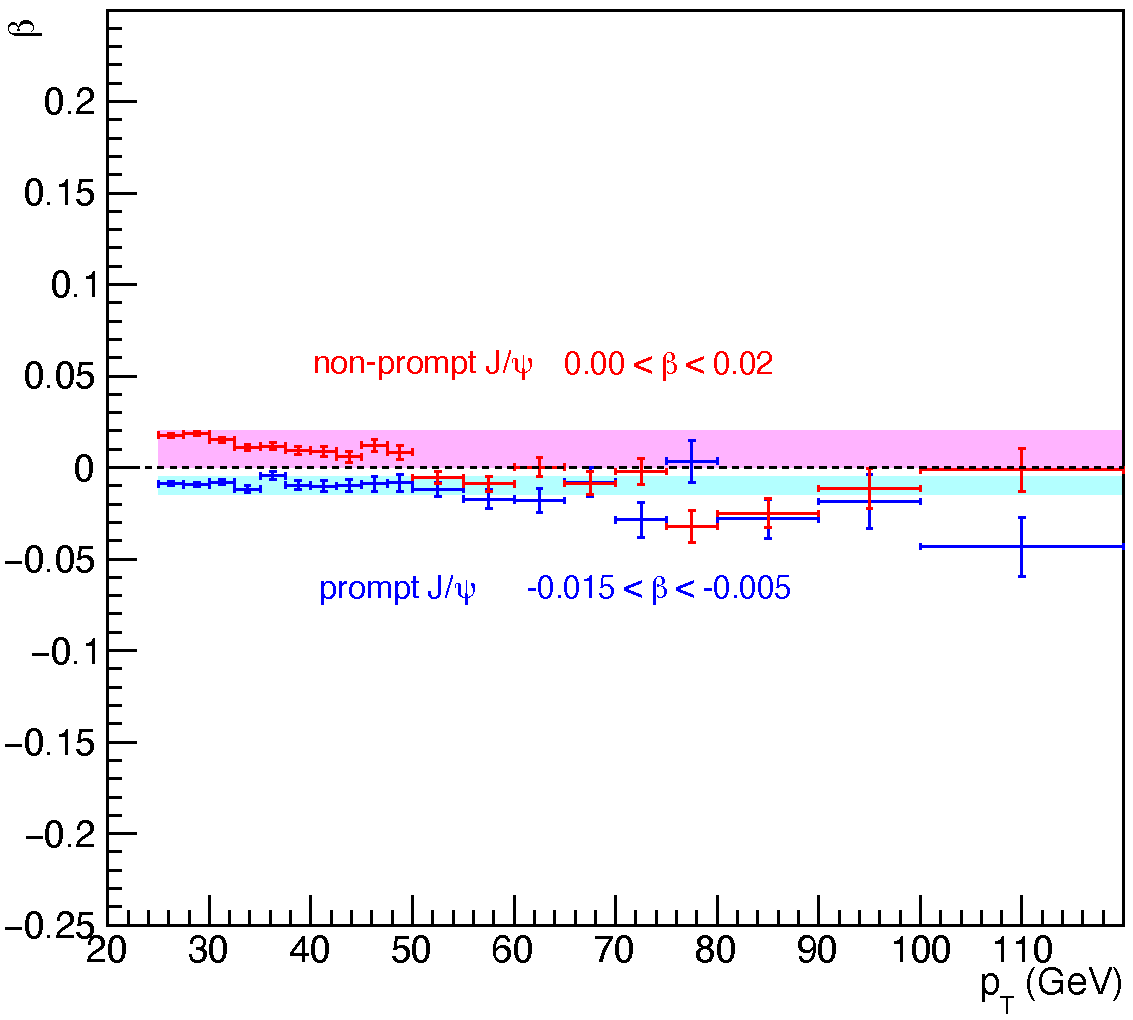
\includegraphics[width=0.48\textwidth]{Figures/chapter6/beta-jpsi.pdf}
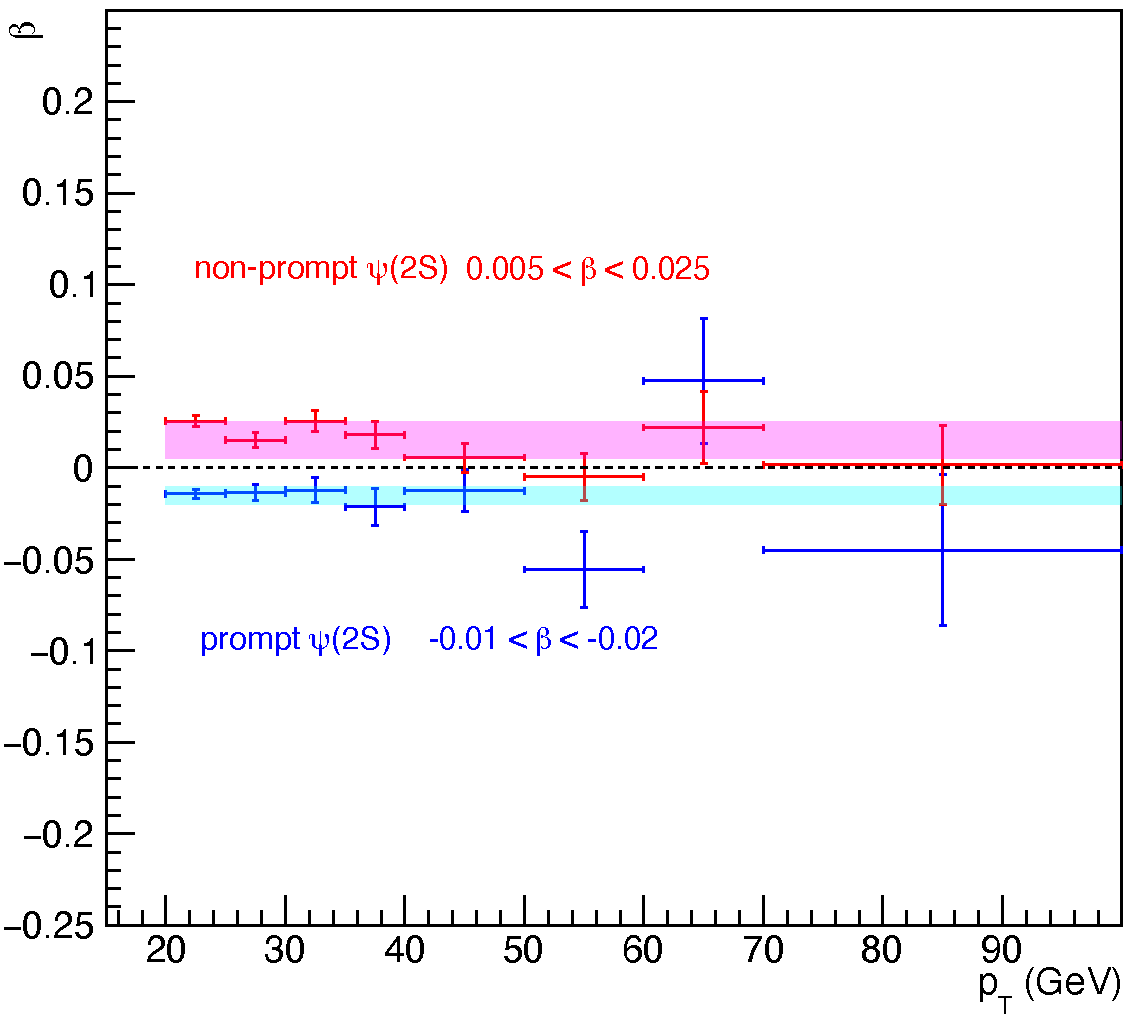
\includegraphics[width=0.48\textwidth]{Figures/chapter6/beta-psip.pdf}
\caption{Fitted $\beta$ values, versus \pt, 
for the prompt (blue) and non-prompt (red) \jpsi (left) and \psip (right) analyses.
The bands represent our estimates for the $\beta$ ranges.}
\label{fig:beta}
\end{figure}

Therefore, the acceptance correction can be made in $\abscosth$,
integrating over the $\varphi$ angle, 
neglecting residual correlations between the two angles.
%
It is worth noting that small non-zero $\beta$ values 
cannot be considered as evidence that there are residual differences 
between the acceptance maps evaluated through the MC simulations
and the real acceptance maps of the actual detector.
In other words, even a perfect MC simulation can lead to 
acceptance-corrected distributions that exhibit small azimuthal anisotropies
in the HX frame.
The reason is that we are using the \emph{proton-proton} HX frame 
and not the \emph{parton-parton} HX frame, 
that would be more suitable to measure the prompt \jpsi polarization.
Similarly, the B meson frame would be more suitable 
to measure the polarization of non-prompt \jpsi mesons.
Since we have no access to those ``natural" frames, 
we must report the measurements in the proton-proton HX frame,
where small azimuthal anisotropies can be expected,
even if they are absent in the ideal frames.

Nevertheless, to be conservative, 
we take the extreme approach of considering that
the residual non-flatness of the $\varphi$ distributions is caused by a 
mismatch between MC and data.
Hence, based on our estimates for the $\beta$ ranges, we compute new $\abscosth$ vs.\ \pt acceptance maps 
reweighing each MC event by the weight $1 + \beta \cdot \cos(2 \varphi)$,
which depends on the $\varphi$ of the event.

\vfill\newpage

The differences between the \lth values obtained with the alternative maps 
(in two extreme options represented by the bands in Fig.~\ref{fig:beta})
and those of the baseline analysis are shown in Fig.~\ref{fig:lth_absDiff_phi},
for the prompt (top) and non-prompt (bottom) \jpsi (left) and \psip (right) analyses.
They are negligible with respect to the grey bands, 
which represent the statistical uncertainty of the baseline results,
so that we could consider this to be a passed check.
Nevertheless, we assign a systematic uncertainty from this source, 
up to 37.5\GeV for the \jpsi case and 35\GeV for the \psip,
computed from the difference between the \lth values 
obtained with the most extreme $\beta$ scenario 
and the baseline values.
This uncertainty is asymmetric but it is quite small
so that we will retain symmetric total systematic uncertainties.

\begin{figure}[t]
\centering
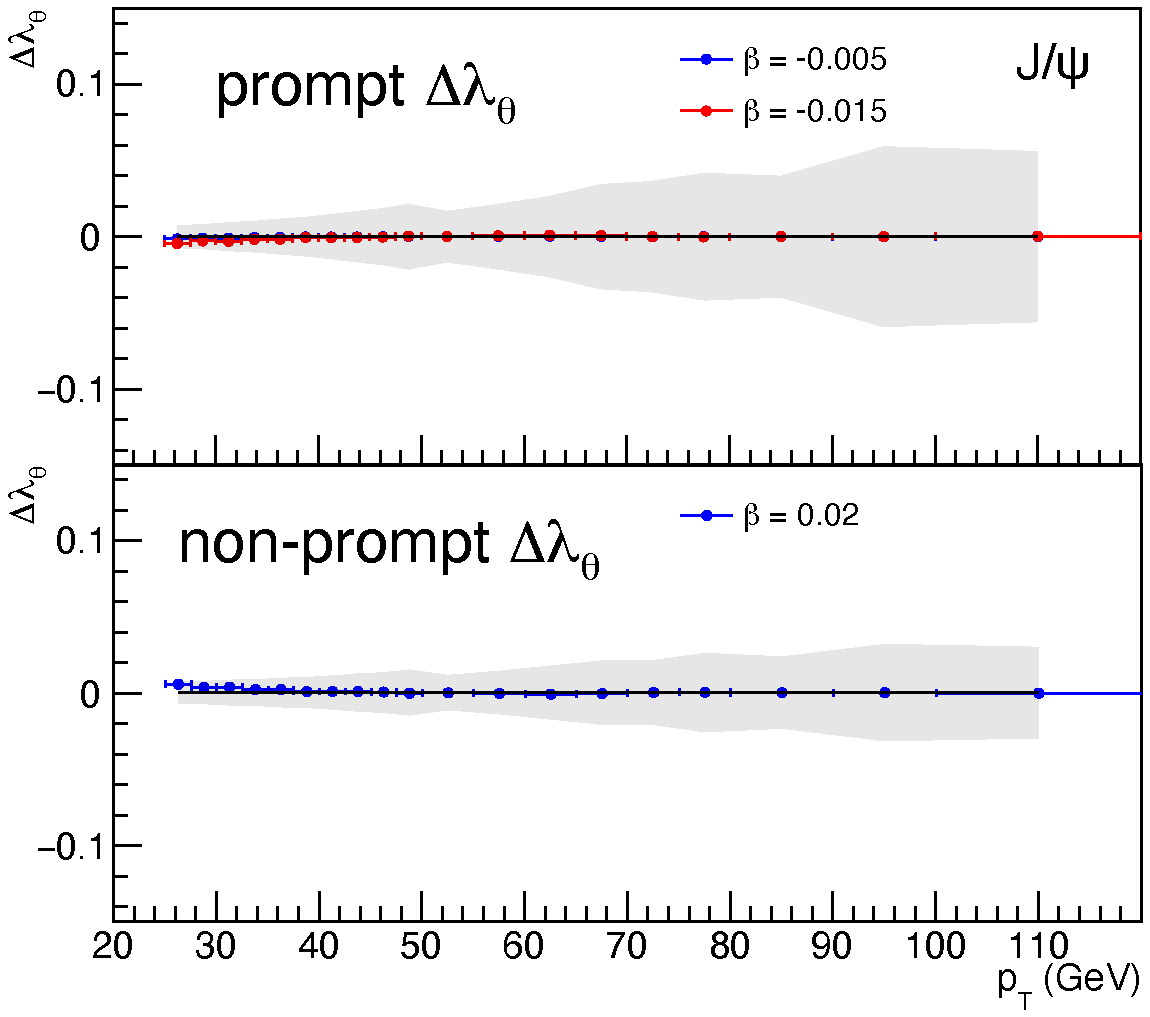
\includegraphics[width=0.48\textwidth]{Figures/chapter6/lth_absDiff_phi_PR_NP-jpsi.pdf}
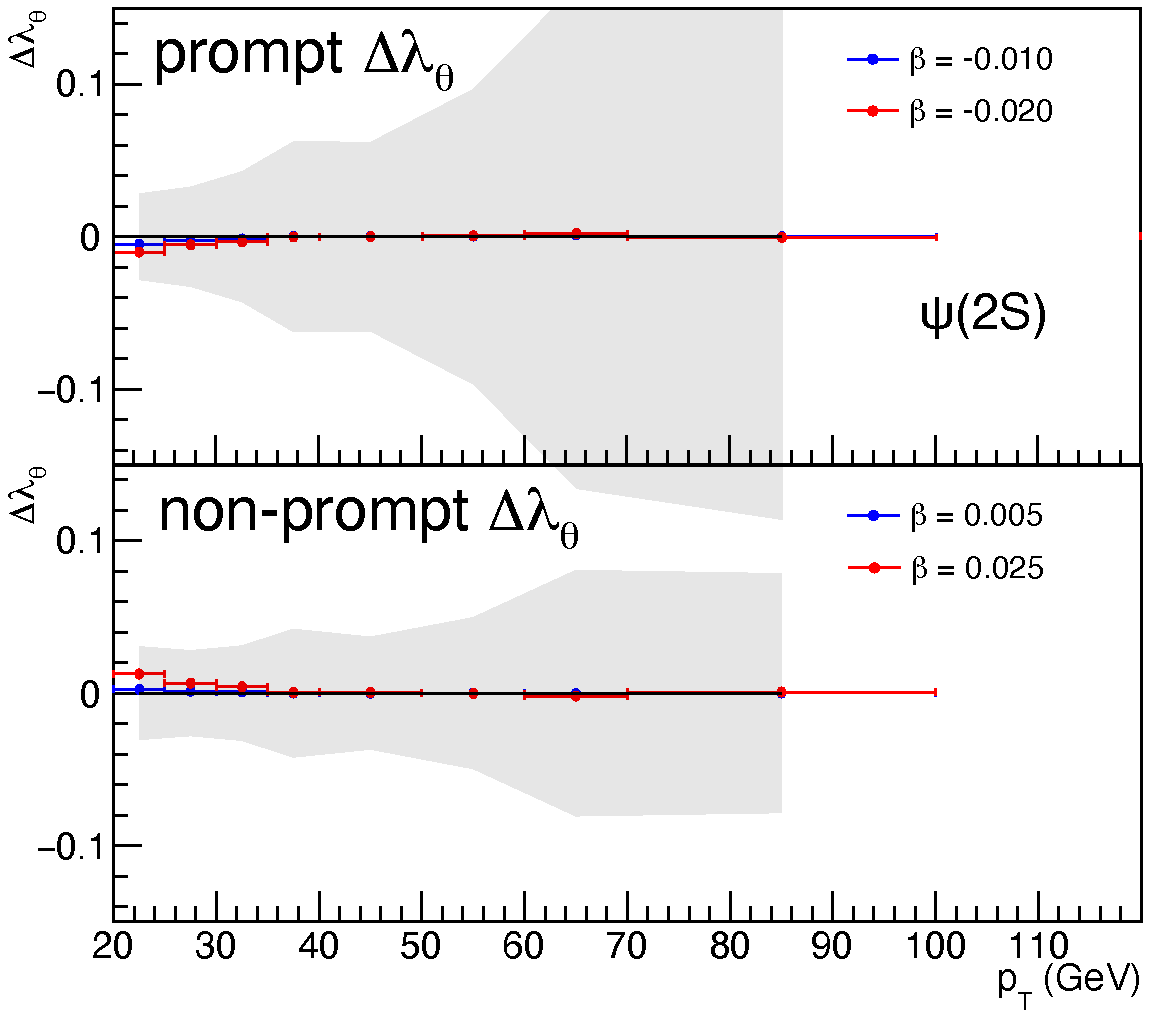
\includegraphics[width=0.48\textwidth]{Figures/chapter6/lth_absDiff_phi_PR_NP-psip.pdf}
\caption{Difference $\Delta \lth$ between the \lth values measured with 
the reweighed acceptance maps 
(using the $\beta$ values mentioned in the legends),
and the baseline values, vs.\ \pt, for the \jpsi (left) and \psip (right) analyses.}
\label{fig:lth_absDiff_phi}
\end{figure}

\vfill\newpage

\subsection{Summary of the systematic uncertainties}

All the uncertainties described in the previous sections of this chapter
are summed in quadrature to give the total 
systematic uncertainty of the measurements.
The squared uncertainties are stacked on the positive hemispheres 
of Fig.~\ref{fig:lth_uncs_stack},
where they can be easily compared with the squared statistical uncertainties,
shown on the negative hemispheres.
This figure shows the results for the non-prompt (left) and prompt (right)
\jpsi (top) and \psip (bottom) measurements.

\begin{figure}[h]
\centering
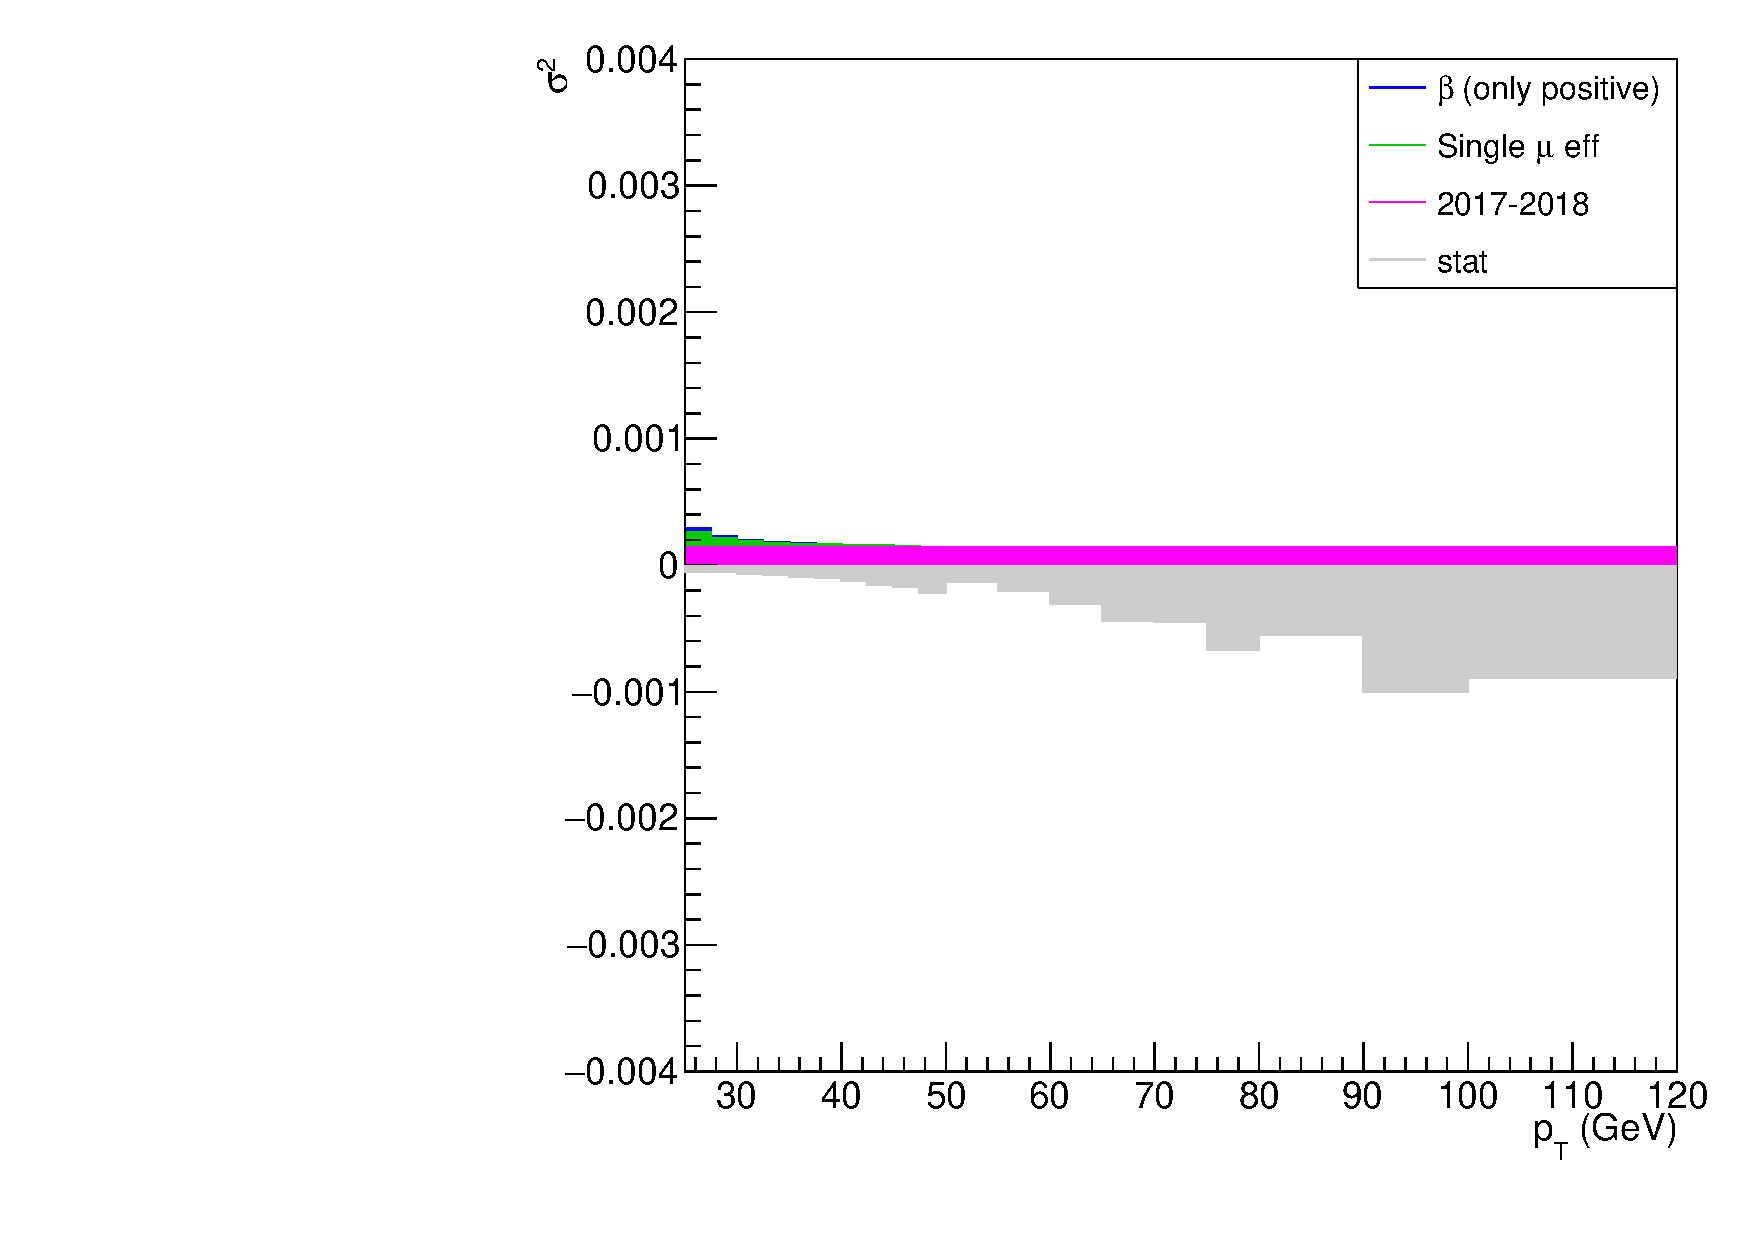
\includegraphics[width=0.48\textwidth]{Figures/chapter6/lthNP_uncs_stack-jpsi.pdf}
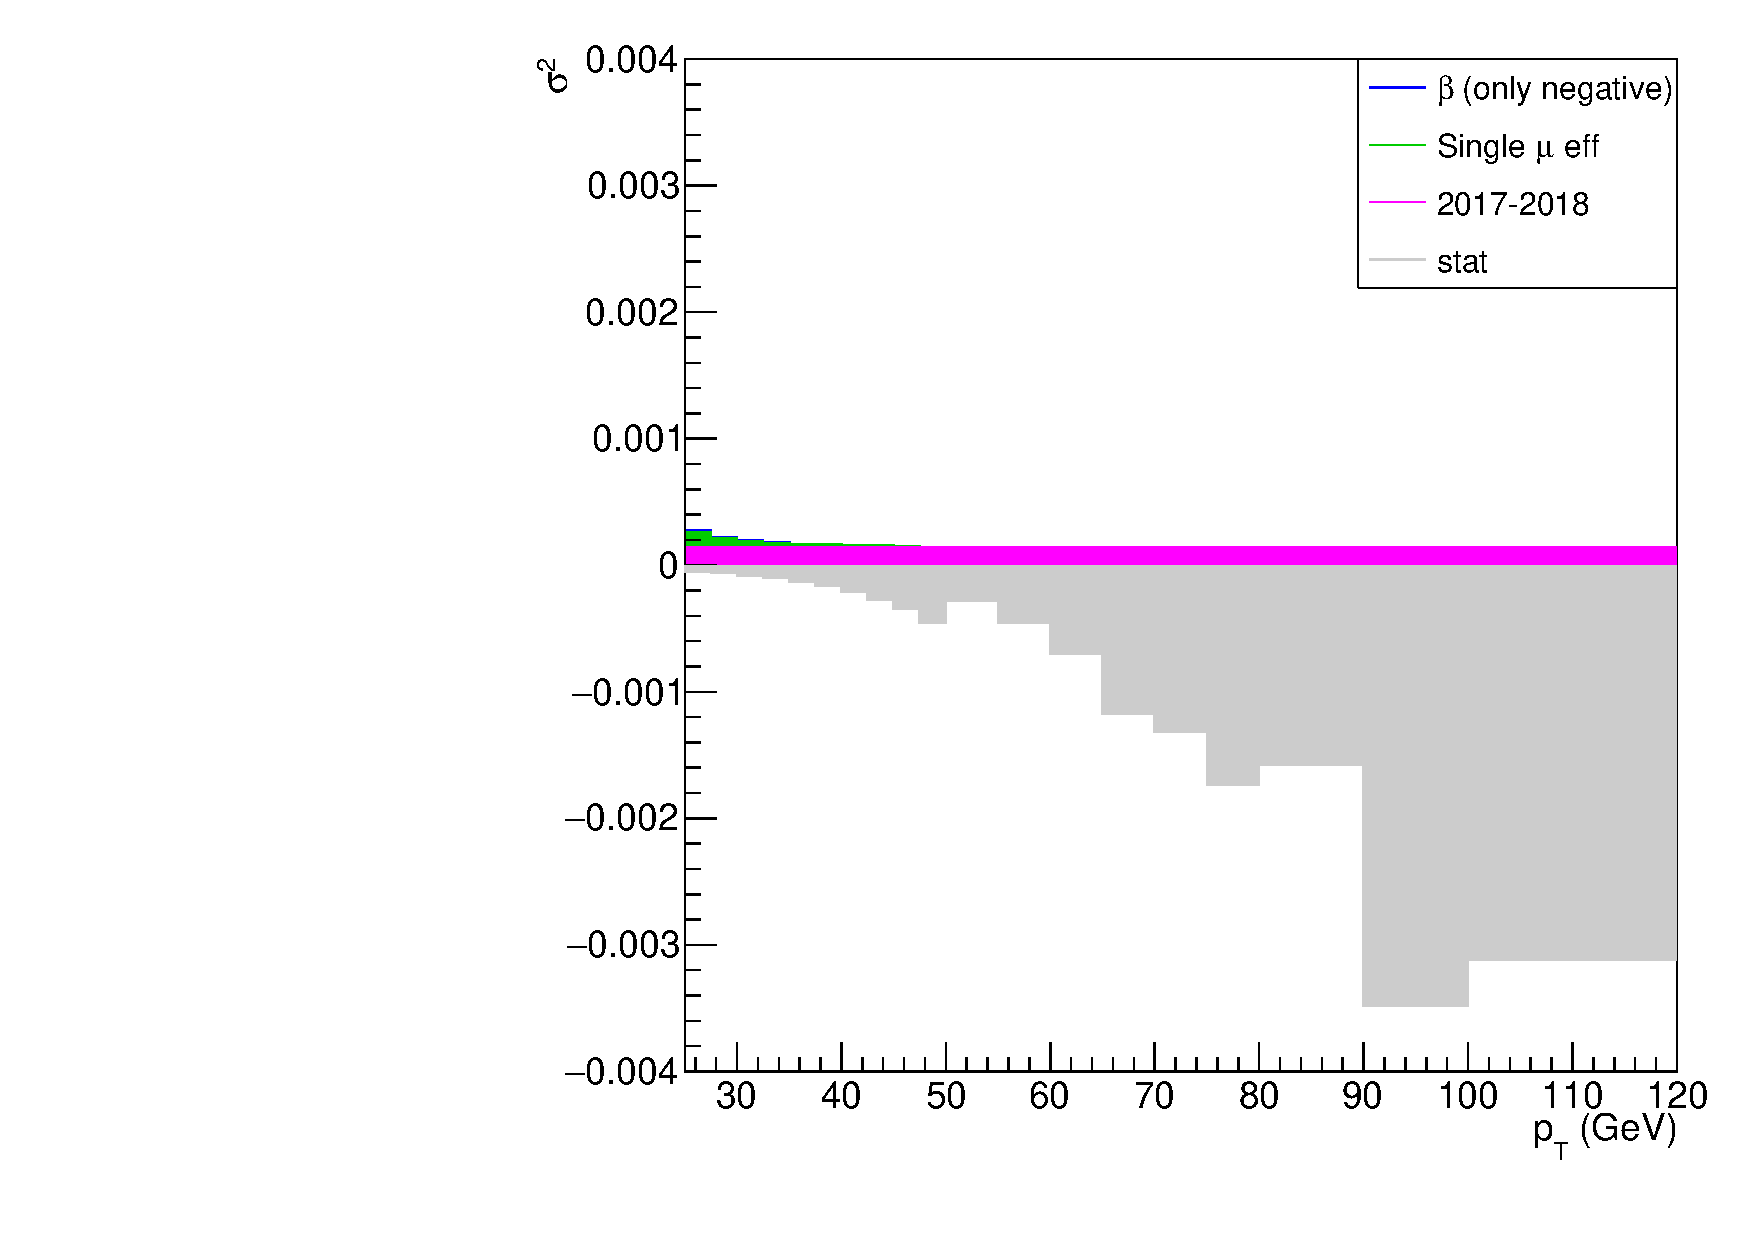
\includegraphics[width=0.48\textwidth]{Figures/chapter6/lthPR_uncs_stack-jpsi.pdf}\\
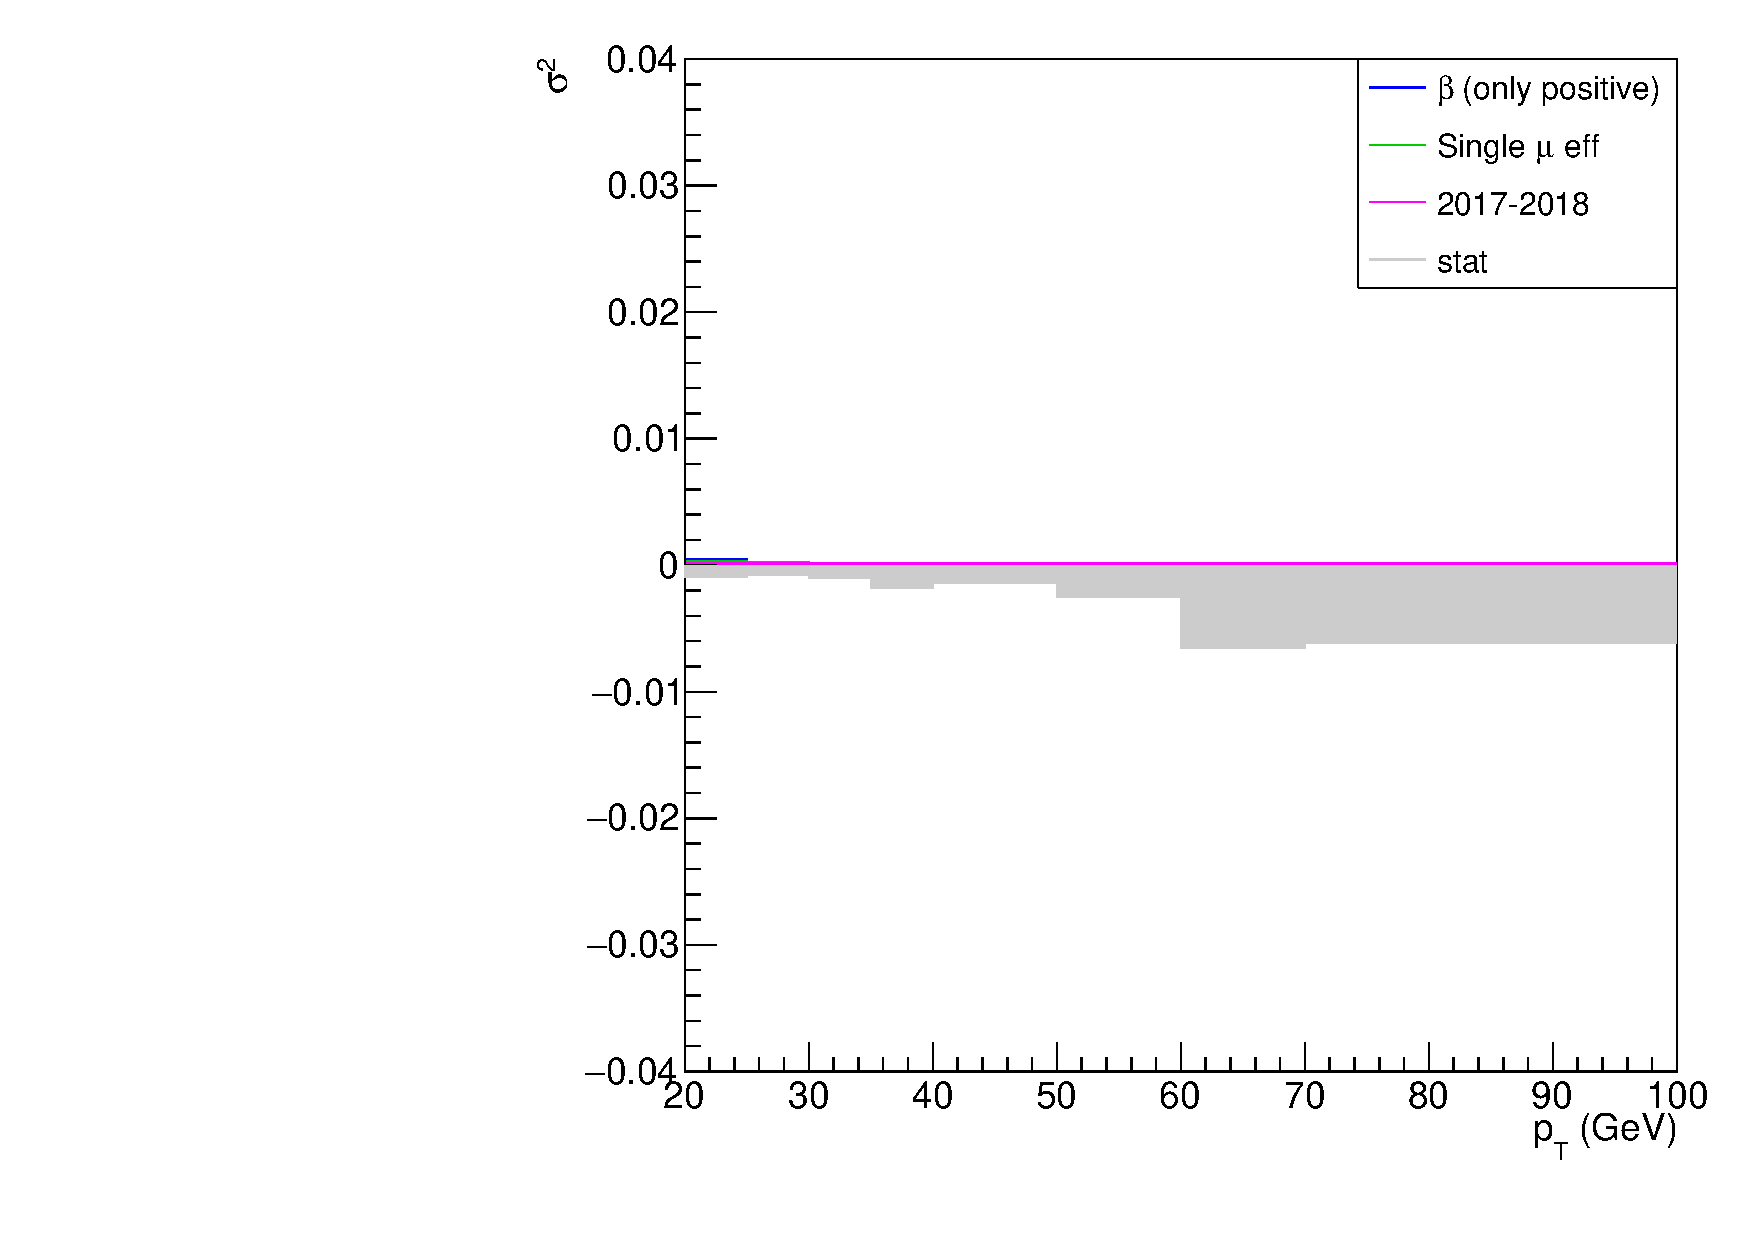
\includegraphics[width=0.48\textwidth]{Figures/chapter6/lthNP_uncs_stack-psip.pdf}
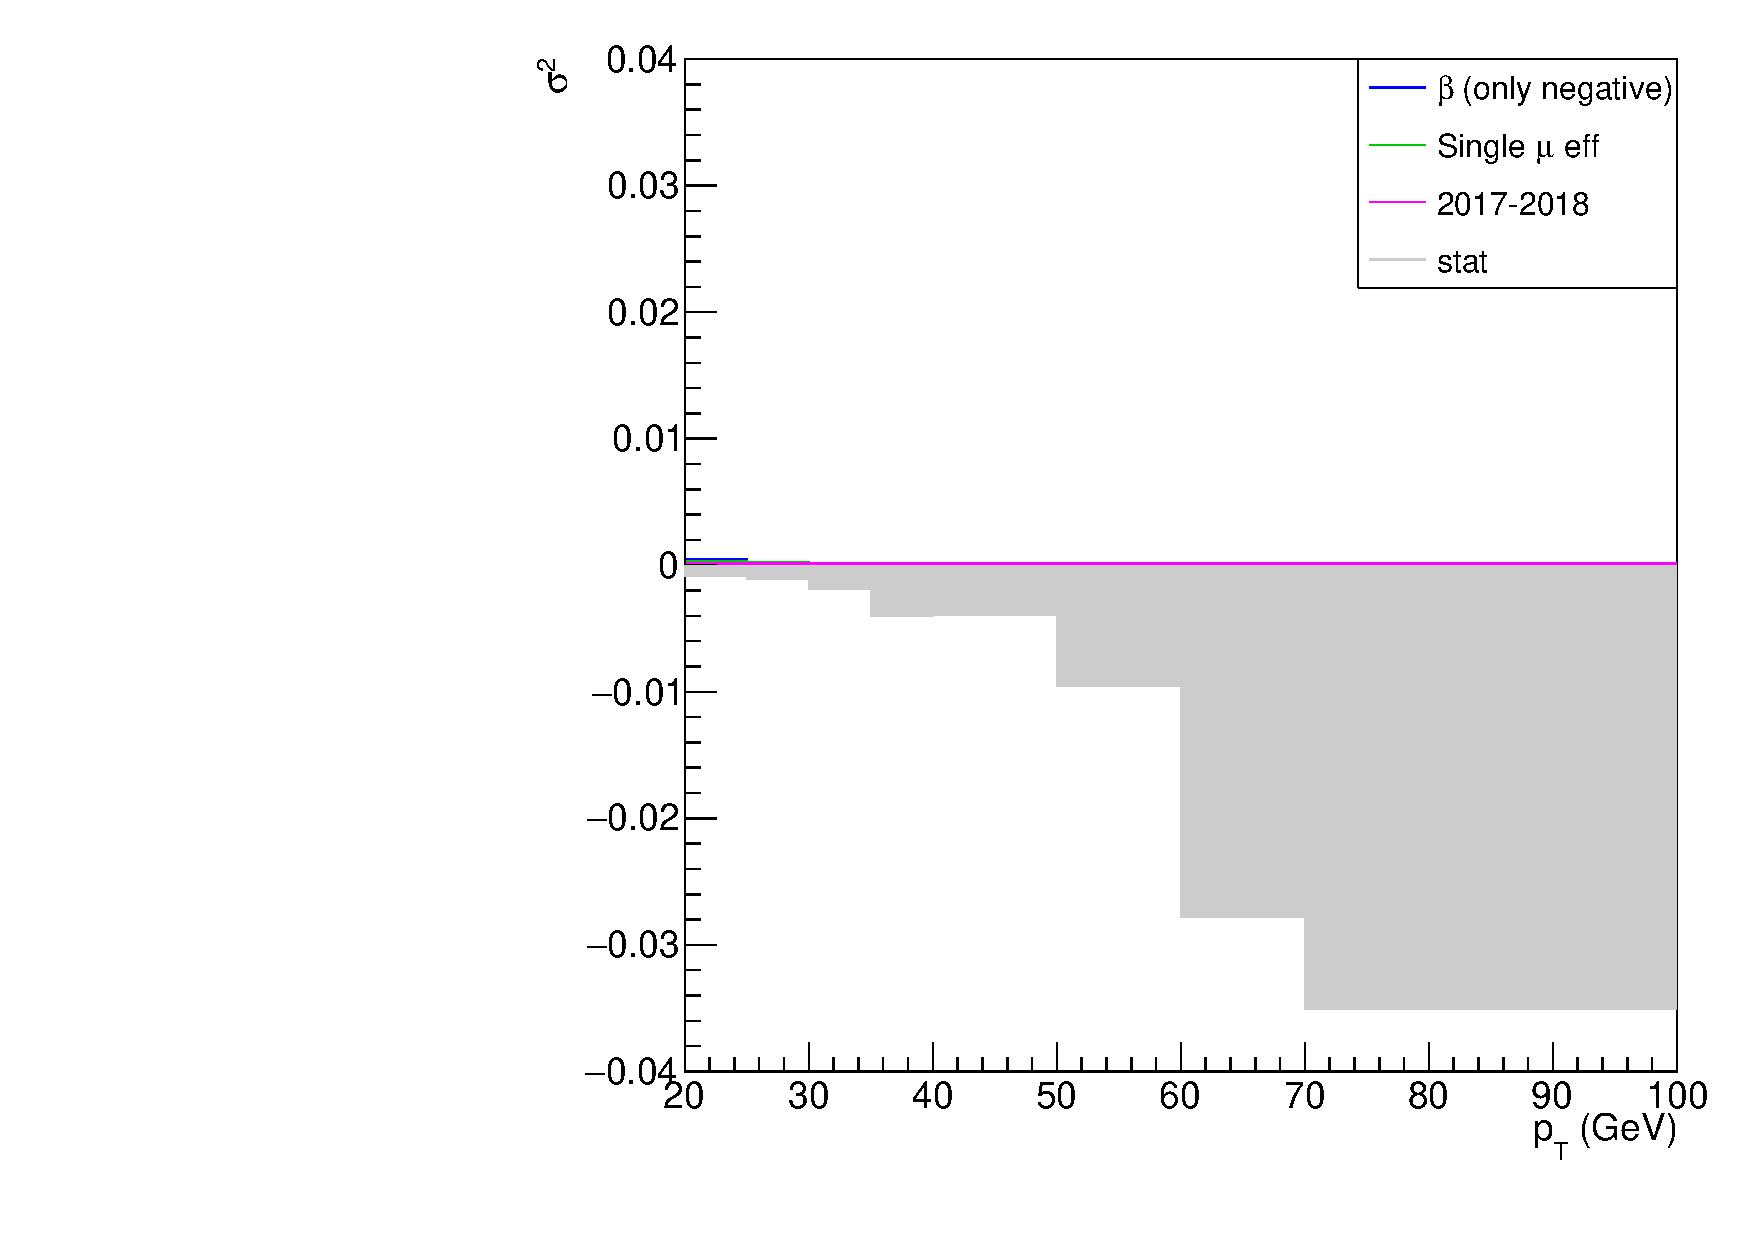
\includegraphics[width=0.48\textwidth]{Figures/chapter6/lthPR_uncs_stack-psip.pdf}
\caption{Systematic uncertainties squared and stacked, on the positive hemisphere, 
and statistical uncertainties squared, on the negative hemisphere, 
for the non-prompt (left) and prompt (right) \jpsi (top) and \psip (bottom) measurements.}
\label{fig:lth_uncs_stack}
\end{figure}

We see that the statistical uncertainties dominate everywhere 
except for \pt smaller than $\sim$\,50\GeV for the \jpsi polarization measurements.

The numerical values of all uncertainties are collected in 
Tables~\ref{tab:syst-jpsiPR}--\ref{tab:syst-psipNP}.

\begin{table}[h]
\centering 
\caption{Systematic uncertainties affecting the prompt \jpsi polarization measurement.}
\label{tab:syst-jpsiPR}
% J/psi Prompt
\begin{tabular}{c|ccc|c}
\pt (GeV) & years & $\mu$ eff.\ & $\beta$ & total \\
\hline
25--27.5 & \multirow{19}{*}{$\pm0.012$} & $\pm0.011$ & $-0.004$ & $\pm0.017$\\
27.5--30 &  & $\pm0.008$ & $-0.003$ & $\pm0.015$\\
30--32.5 &  & $\pm0.007$ & $-0.003$ & $\pm0.014$\\
32.5--35 &  & $\pm0.006$ & $-0.002$ & $\pm0.013$\\
35--37.5 &  & $\pm0.005$ & $-0.002$ & $\pm0.013$\\
37.5--40 &  & $\pm0.004$ & $-$ & $\pm0.013$\\
40--42.5 &  & $\pm0.004$ & $-$ & $\pm0.013$\\
42.5--45 &  & $\pm0.003$ & $-$ & $\pm0.012$\\
45--47.5 &  & $\pm0.002$ & $-$ & $\pm0.012$\\
47.5--50 &  & $\pm0.001$ & $-$ & $\pm0.012$\\
50--55 &  & $-$ & $-$ & $\pm0.012$\\
55--60 &  & $-$ & $-$ & $\pm0.012$\\
60--65 &  & $-$ & $-$ & $\pm0.012$\\
65--70 &  & $-$ & $-$ & $\pm0.012$\\
70--75 &  & $-$ & $-$ & $\pm0.012$\\
75--80 &  & $-$ & $-$ & $\pm0.012$\\
80--90 &  & $-$ & $-$ & $\pm0.012$\\
90--100 &  & $-$ & $-$ & $\pm0.012$\\
100--120 &  & $-$ & $-$ & $\pm0.012$
\end{tabular}
\end{table}

\begin{table}[h]
\centering 
\caption{Systematic uncertainties affecting the non-prompt \jpsi polarization measurement.}
\label{tab:syst-jpsiNP}
% J/psi Non-Prompt
\begin{tabular}{c|ccc|c}
\pt (GeV) & years & $\mu$ eff.\ & $\beta$ & total \\
\hline
25--27.5 & \multirow{19}{*}{$\pm0.012$} & $\pm0.011$ & $+0.005$ & $\pm0.017$\\
27.5--30 &  & $\pm0.008$ & $+0.003$ & $\pm0.015$\\
30--32.5 &  & $\pm0.007$ & $+0.004$ & $\pm0.014$\\
32.5--35 &  & $\pm0.006$ & $+0.002$ & $\pm0.013$\\
35--37.5 &  & $\pm0.005$ & $+0.002$ & $\pm0.013$\\
37.5--40 &  & $\pm0.004$ & $-$ & $\pm0.013$\\
40--42.5 &  & $\pm0.004$ & $-$ & $\pm0.013$\\
42.5--45 &  & $\pm0.003$ & $-$ & $\pm0.012$\\
45--47.5 &  & $\pm0.002$ & $-$ & $\pm0.012$\\
47.5--50 &  & $\pm0.001$ & $-$ & $\pm0.012$\\
50--55 &  & $-$ & $-$ & $\pm0.012$\\
55--60 &  & $-$ & $-$ & $\pm0.012$\\
60--65 &  & $-$ & $-$ & $\pm0.012$\\
65--70 &  & $-$ & $-$ & $\pm0.012$\\
70--75 &  & $-$ & $-$ & $\pm0.012$\\
75--80 &  & $-$ & $-$ & $\pm0.012$\\
80--90 &  & $-$ & $-$ & $\pm0.012$\\
90--100 &  & $-$ & $-$ & $\pm0.012$\\
100--120 &  & $-$ & $-$ & $\pm0.012$
\end{tabular}
\end{table}

\begin{table}[h]
\centering 
\caption{Systematic uncertainties affecting the prompt \psip polarization measurement.}
\label{tab:syst-psipPR}
% psi(2S) Prompt
\begin{tabular}{c|ccc|c}
\pt (GeV) & years & $\mu$ eff.\ & $\beta$ & total \\
\hline
20--25 & \multirow{8}{*}{$\pm0.012$} & $\pm0.014$ & $-0.010$ & $\pm0.021$\\
25--30 &  & $\pm0.008$ & $-0.006$ & $\pm0.016$\\
30--35 &  & $\pm0.005$ & $-0.004$ & $\pm0.013$\\
35--40 &  & $\pm0.001$ & $-$ & $\pm0.012$\\
40--50 &  & $-$ & $-$ & $\pm0.012$\\
50--60 &  & $-$ & $-$ & $\pm0.012$\\
60--70 &  & $-$ & $-$ & $\pm0.012$\\
70--100 &  & $-$ & $-$ & $\pm0.012$
\end{tabular}
\end{table}

\begin{table}[h]
\centering 
\caption{Systematic uncertainties affecting the non-prompt \psip polarization measurement.}
\label{tab:syst-psipNP}
% psi(2S) Non-Prompt
\begin{tabular}{c|ccc|c}
\pt (GeV) & years & $\mu$ eff.\ & $\beta$ & total \\
\hline
20--25 & \multirow{8}{*}{$\pm0.012$} & $\pm0.014$ & $+0.013$ & $\pm0.023$\\
25--30 &  & $\pm0.008$ & $+0.007$ & $\pm0.016$\\
30--35 &  & $\pm0.005$ & $+0.004$ & $\pm0.014$\\
35--40 &  & $\pm0.001$ & $-$ & $\pm0.012$\\
40--50 &  & $-$ & $-$ & $\pm0.012$\\
50--60 &  & $-$ & $-$ & $\pm0.012$\\
60--70 &  & $-$ & $-$ & $\pm0.012$\\
70--100 &  & $-$ & $-$ & $\pm0.012$
\end{tabular}
\end{table}

